\documentclass[twoside]{book}

% Packages required by doxygen
\usepackage{fixltx2e}
\usepackage{calc}
\usepackage{doxygen}
\usepackage[export]{adjustbox} % also loads graphicx
\usepackage{graphicx}
\usepackage[utf8]{inputenc}
\usepackage{makeidx}
\usepackage{multicol}
\usepackage{multirow}
\PassOptionsToPackage{warn}{textcomp}
\usepackage{textcomp}
\usepackage[nointegrals]{wasysym}
\usepackage[table]{xcolor}

% Font selection
\usepackage[T1]{fontenc}
\usepackage[scaled=.90]{helvet}
\usepackage{courier}
\usepackage{amssymb}
\usepackage{sectsty}
\renewcommand{\familydefault}{\sfdefault}
\allsectionsfont{%
  \fontseries{bc}\selectfont%
  \color{darkgray}%
}
\renewcommand{\DoxyLabelFont}{%
  \fontseries{bc}\selectfont%
  \color{darkgray}%
}
\newcommand{\+}{\discretionary{\mbox{\scriptsize$\hookleftarrow$}}{}{}}

% Page & text layout
\usepackage{geometry}
\geometry{%
  a4paper,%
  top=2.5cm,%
  bottom=2.5cm,%
  left=2.5cm,%
  right=2.5cm%
}
\tolerance=750
\hfuzz=15pt
\hbadness=750
\setlength{\emergencystretch}{15pt}
\setlength{\parindent}{0cm}
\setlength{\parskip}{3ex plus 2ex minus 2ex}
\makeatletter
\renewcommand{\paragraph}{%
  \@startsection{paragraph}{4}{0ex}{-1.0ex}{1.0ex}{%
    \normalfont\normalsize\bfseries\SS@parafont%
  }%
}
\renewcommand{\subparagraph}{%
  \@startsection{subparagraph}{5}{0ex}{-1.0ex}{1.0ex}{%
    \normalfont\normalsize\bfseries\SS@subparafont%
  }%
}
\makeatother

% Headers & footers
\usepackage{fancyhdr}
\pagestyle{fancyplain}
\fancyhead[LE]{\fancyplain{}{\bfseries\thepage}}
\fancyhead[CE]{\fancyplain{}{}}
\fancyhead[RE]{\fancyplain{}{\bfseries\leftmark}}
\fancyhead[LO]{\fancyplain{}{\bfseries\rightmark}}
\fancyhead[CO]{\fancyplain{}{}}
\fancyhead[RO]{\fancyplain{}{\bfseries\thepage}}
\fancyfoot[LE]{\fancyplain{}{}}
\fancyfoot[CE]{\fancyplain{}{}}
\fancyfoot[RE]{\fancyplain{}{\bfseries\scriptsize Generated by Doxygen }}
\fancyfoot[LO]{\fancyplain{}{\bfseries\scriptsize Generated by Doxygen }}
\fancyfoot[CO]{\fancyplain{}{}}
\fancyfoot[RO]{\fancyplain{}{}}
\renewcommand{\footrulewidth}{0.4pt}
\renewcommand{\chaptermark}[1]{%
  \markboth{#1}{}%
}
\renewcommand{\sectionmark}[1]{%
  \markright{\thesection\ #1}%
}

% Indices & bibliography
\usepackage{natbib}
\usepackage[titles]{tocloft}
\setcounter{tocdepth}{3}
\setcounter{secnumdepth}{5}
\makeindex

% Hyperlinks (required, but should be loaded last)
\usepackage{ifpdf}
\ifpdf
  \usepackage[pdftex,pagebackref=true]{hyperref}
\else
  \usepackage[ps2pdf,pagebackref=true]{hyperref}
\fi
\hypersetup{%
  colorlinks=true,%
  linkcolor=blue,%
  citecolor=blue,%
  unicode%
}

% Custom commands
\newcommand{\clearemptydoublepage}{%
  \newpage{\pagestyle{empty}\cleardoublepage}%
}

\usepackage{caption}
\captionsetup{labelsep=space,justification=centering,font={bf},singlelinecheck=off,skip=4pt,position=top}

%===== C O N T E N T S =====

\begin{document}

% Titlepage & ToC
\hypersetup{pageanchor=false,
             bookmarksnumbered=true,
             pdfencoding=unicode
            }
\pagenumbering{alph}
\begin{titlepage}
\vspace*{7cm}
\begin{center}%
{\Large My Project }\\
\vspace*{1cm}
{\large Generated by Doxygen 1.8.13}\\
\end{center}
\end{titlepage}
\clearemptydoublepage
\pagenumbering{roman}
\tableofcontents
\clearemptydoublepage
\pagenumbering{arabic}
\hypersetup{pageanchor=true}

%--- Begin generated contents ---
\chapter{library documentation}
\label{index}\hypertarget{index}{}\hypertarget{index_Author}{}\section{Author}\label{index_Author}
Duur Alblas (c) 2019~\newline
\href{mailto:duur.alblas@student.hu.nl}{\tt duur.\+alblas@student.\+hu.\+nl} \hypertarget{index_Version}{}\section{Version}\label{index_Version}
Version 1.\+0 (last modified 5 july 2019) \hypertarget{index_Copyright}{}\section{Copyright}\label{index_Copyright}
Boost license All D\&D related references belong to Wizards of the Coast L\+LC 
\chapter{Character Card}
\label{md_README}
\Hypertarget{md_README}
Author \+: Duur Alblas (c) 2019 \href{mailto:duur.alblas@student.hu.nl}{\tt duur.\+alblas@student.\+hu.\+nl}

This Library contains support for a R\+C522 chip and a M\+I\+F\+A\+RE 1K card version M\+F1\+S503yX.

It is relatively easily expandable to support other chip using S\+PI or even I2C or U\+A\+RT.

You can also implement support for more M\+I\+F\+A\+RE card versiona and even other cards.

With some minor adjustments you can also support different games using character sheets.

Version 1.\+0 (last modified 5 july 2019)

section Copyright

Boost license (See accompanying file L\+I\+C\+E\+N\+S\+E\+\_\+1\+\_\+0.\+txt or copy at \href{http://www.boost.org/LICENSE_1_0.txt}{\tt http\+://www.\+boost.\+org/\+L\+I\+C\+E\+N\+S\+E\+\_\+1\+\_\+0.\+txt})

All D\&D related references belong to Wizards of the Coast L\+LC 
\chapter{Hierarchical Index}
\section{Class Hierarchy}
This inheritance list is sorted roughly, but not completely, alphabetically\+:\begin{DoxyCompactList}
\item \contentsline{section}{mifare\+:\+:card}{\pageref{classmifare_1_1card}}{}
\item \contentsline{section}{sheet}{\pageref{classsheet}}{}
\item \contentsline{section}{spi\+Reader}{\pageref{classspiReader}}{}
\begin{DoxyCompactList}
\item \contentsline{section}{rc522}{\pageref{classrc522}}{}
\end{DoxyCompactList}
\end{DoxyCompactList}

\chapter{Class Index}
\section{Class List}
Here are the classes, structs, unions and interfaces with brief descriptions\+:\begin{DoxyCompactList}
\item\contentsline{section}{\hyperlink{classmifare_1_1card}{mifare\+::card} \\*A card class for mifare cards }{\pageref{classmifare_1_1card}}{}
\item\contentsline{section}{\hyperlink{classrc522}{rc522} \\*Rc522 chip class inherits from \hyperlink{classspiReader}{spi\+Reader} }{\pageref{classrc522}}{}
\item\contentsline{section}{\hyperlink{classsheet}{sheet} \\*A class to contain character sheet data }{\pageref{classsheet}}{}
\item\contentsline{section}{\hyperlink{classspiReader}{spi\+Reader} \\*Spi\+Reader A\+DT class }{\pageref{classspiReader}}{}
\end{DoxyCompactList}

\chapter{Class Documentation}
\hypertarget{classmifare_1_1card}{}\section{mifare\+:\+:card Class Reference}
\label{classmifare_1_1card}\index{mifare\+::card@{mifare\+::card}}


A card class for mifare cards.  




{\ttfamily \#include $<$supp.\+hpp$>$}

\subsection*{Public Member Functions}
\begin{DoxyCompactItemize}
\item 
\mbox{\Hypertarget{classmifare_1_1card_add87ee9228a95ef57e6778e837a5fa68}\label{classmifare_1_1card_add87ee9228a95ef57e6778e837a5fa68}} 
\hyperlink{classmifare_1_1card_add87ee9228a95ef57e6778e837a5fa68}{card} (std\+::array$<$ uint8\+\_\+t, 4 $>$ \hyperlink{classmifare_1_1card_a0f97900bf64b956ac9f9622671aa4f74}{uid}, std\+::array$<$ uint8\+\_\+t, 6 $>$ \hyperlink{classmifare_1_1card_a9d6bb609c82ca6fa65a79e83656db964}{keyA}, std\+::array$<$ uint8\+\_\+t, 6 $>$ \hyperlink{classmifare_1_1card_ae99191bf1a9478b61f4b0043c6e0d7bf}{keyB}, uint8\+\_\+t \hyperlink{classmifare_1_1card_a3283a205a271075bd6e4b0bea3f015cb}{max\+Blocks})
\begin{DoxyCompactList}\small\item\em A constructor with some default values  This constructor can be called without supplying all the parameters because default values have been supplied. \end{DoxyCompactList}\item 
\mbox{\Hypertarget{classmifare_1_1card_aff06c5ecc67800474ee8f3e76d4bf1f4}\label{classmifare_1_1card_aff06c5ecc67800474ee8f3e76d4bf1f4}} 
\hyperlink{classmifare_1_1card_aff06c5ecc67800474ee8f3e76d4bf1f4}{card} ()
\begin{DoxyCompactList}\small\item\em Default constructor  This constructor doesn\textquotesingle{}t need any input and only has default values. \end{DoxyCompactList}\end{DoxyCompactItemize}
\subsection*{Public Attributes}
\begin{DoxyCompactItemize}
\item 
std\+::array$<$ uint8\+\_\+t, 4 $>$ \hyperlink{classmifare_1_1card_a0f97900bf64b956ac9f9622671aa4f74}{uid}
\begin{DoxyCompactList}\small\item\em A array for the U\+ID (N\+U\+ID) \end{DoxyCompactList}\item 
std\+::array$<$ uint8\+\_\+t, 6 $>$ \hyperlink{classmifare_1_1card_a9d6bb609c82ca6fa65a79e83656db964}{keyA}
\begin{DoxyCompactList}\small\item\em A array for Key A. \end{DoxyCompactList}\item 
std\+::array$<$ uint8\+\_\+t, 6 $>$ \hyperlink{classmifare_1_1card_ae99191bf1a9478b61f4b0043c6e0d7bf}{keyB}
\begin{DoxyCompactList}\small\item\em A array for Key B. \end{DoxyCompactList}\item 
uint8\+\_\+t \hyperlink{classmifare_1_1card_a3283a205a271075bd6e4b0bea3f015cb}{max\+Blocks}
\begin{DoxyCompactList}\small\item\em The maximum amount of blocks available. \end{DoxyCompactList}\end{DoxyCompactItemize}


\subsection{Detailed Description}
A card class for mifare cards. 

This class stores data associated with a mifare card.~\newline
For now this class supports only the M\+F1\+S503yX type of the mifare cards,~\newline
but is relatively easily expandable. 

\subsection{Member Data Documentation}
\mbox{\Hypertarget{classmifare_1_1card_a9d6bb609c82ca6fa65a79e83656db964}\label{classmifare_1_1card_a9d6bb609c82ca6fa65a79e83656db964}} 
\index{mifare\+::card@{mifare\+::card}!keyA@{keyA}}
\index{keyA@{keyA}!mifare\+::card@{mifare\+::card}}
\subsubsection{\texorpdfstring{keyA}{keyA}}
{\footnotesize\ttfamily std\+::array$<$uint8\+\_\+t,6$>$ mifare\+::card\+::keyA}



A array for Key A. 

We store Key A in this array with a maximum size of 6 bytes. \mbox{\Hypertarget{classmifare_1_1card_ae99191bf1a9478b61f4b0043c6e0d7bf}\label{classmifare_1_1card_ae99191bf1a9478b61f4b0043c6e0d7bf}} 
\index{mifare\+::card@{mifare\+::card}!keyB@{keyB}}
\index{keyB@{keyB}!mifare\+::card@{mifare\+::card}}
\subsubsection{\texorpdfstring{keyB}{keyB}}
{\footnotesize\ttfamily std\+::array$<$uint8\+\_\+t,6$>$ mifare\+::card\+::keyB}



A array for Key B. 

We store Key B in this array with a maximum size of 6 bytes. \mbox{\Hypertarget{classmifare_1_1card_a3283a205a271075bd6e4b0bea3f015cb}\label{classmifare_1_1card_a3283a205a271075bd6e4b0bea3f015cb}} 
\index{mifare\+::card@{mifare\+::card}!max\+Blocks@{max\+Blocks}}
\index{max\+Blocks@{max\+Blocks}!mifare\+::card@{mifare\+::card}}
\subsubsection{\texorpdfstring{max\+Blocks}{maxBlocks}}
{\footnotesize\ttfamily uint8\+\_\+t mifare\+::card\+::max\+Blocks}



The maximum amount of blocks available. 

We store the value of the maximum amount of avaiable blocks here.~\newline
Because we only support the M\+F1\+S503yX max\+Blocks is 64 by default. \mbox{\Hypertarget{classmifare_1_1card_a0f97900bf64b956ac9f9622671aa4f74}\label{classmifare_1_1card_a0f97900bf64b956ac9f9622671aa4f74}} 
\index{mifare\+::card@{mifare\+::card}!uid@{uid}}
\index{uid@{uid}!mifare\+::card@{mifare\+::card}}
\subsubsection{\texorpdfstring{uid}{uid}}
{\footnotesize\ttfamily std\+::array$<$uint8\+\_\+t,4$>$ mifare\+::card\+::uid}



A array for the U\+ID (N\+U\+ID) 

We store the U\+ID (N\+U\+ID in the case of M\+F1\+S503yX) with a maximum size of 4 bytes. 

The documentation for this class was generated from the following files\+:\begin{DoxyCompactItemize}
\item 
supp.\+hpp\item 
supp.\+cpp\end{DoxyCompactItemize}

\hypertarget{classrc522}{}\section{rc522 Class Reference}
\label{classrc522}\index{rc522@{rc522}}


\hyperlink{classrc522}{rc522} chip class inherits from \hyperlink{classspiReader}{spi\+Reader}  




{\ttfamily \#include $<$rc522.\+hpp$>$}



Inheritance diagram for rc522\+:
\nopagebreak
\begin{figure}[H]
\begin{center}
\leavevmode
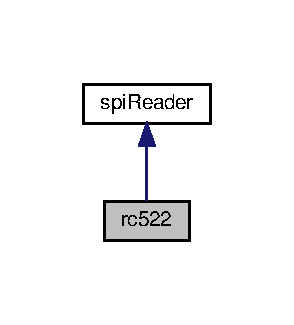
\includegraphics[width=141pt]{classrc522__inherit__graph}
\end{center}
\end{figure}


Collaboration diagram for rc522\+:
\nopagebreak
\begin{figure}[H]
\begin{center}
\leavevmode
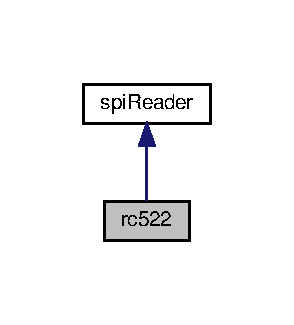
\includegraphics[width=141pt]{classrc522__coll__graph}
\end{center}
\end{figure}
\subsection*{Public Types}
\begin{DoxyCompactItemize}
\item 
enum \hyperlink{classrc522_a83057db5f8fefa3dc9a6e8e5f0e191ee}{registers} \{ \newline
{\bfseries Reserved\+\_\+00} = 0x00, 
{\bfseries Command\+Reg} = 0x01, 
{\bfseries Coml\+En\+Reg} = 0x02, 
{\bfseries Divl\+En\+Reg} = 0x03, 
\newline
{\bfseries Com\+Irq\+Reg} = 0x04, 
{\bfseries Div\+Irq\+Reg} = 0x05, 
{\bfseries Error\+Reg} = 0x06, 
{\bfseries Status1\+Reg} = 0x07, 
\newline
{\bfseries Status2\+Reg} = 0x08, 
{\bfseries F\+I\+F\+O\+Data\+Reg} = 0x09, 
{\bfseries F\+I\+F\+O\+Level\+Reg} = 0x0A, 
{\bfseries Water\+Level\+Reg} = 0x0B, 
\newline
{\bfseries Control\+Reg} = 0x0C, 
{\bfseries Bit\+Framing\+Reg} = 0x0D, 
{\bfseries Coll\+Reg} = 0x0E, 
{\bfseries Reserved\+\_\+0F} = 0x0F
 \}\begin{DoxyCompactList}\small\item\em A enum class with Addressable Registers. \end{DoxyCompactList}
\item 
enum \hyperlink{classrc522_a3a205976fb9b7265bc5b7971215fbb7c}{reg\+Commands} \{ \newline
{\bfseries Idle} = 0x00, 
{\bfseries Mem} = 0x01, 
{\bfseries Generate\+Random\+ID} = 0x02, 
{\bfseries Calc\+C\+RC} = 0x03, 
\newline
{\bfseries Transmit} = 0x04, 
{\bfseries No\+Cmd\+Change} = 0x07, 
{\bfseries Receive} = 0x08, 
{\bfseries Transceive} = 0x0C, 
\newline
{\bfseries Reserved} = 0x0D, 
{\bfseries M\+F\+Authent} = 0x0E, 
{\bfseries Soft\+Reset} = 0x0F
 \}\begin{DoxyCompactList}\small\item\em A enum class with register commands for the Command\+Reg. \end{DoxyCompactList}
\item 
enum \hyperlink{classrc522_a6df2359c88d6c2f47faf58bc9e09eaa4}{commands} \{ \newline
{\bfseries Reserved\+\_\+10} = 0x10, 
{\bfseries Mode\+Reg} = 0x11, 
{\bfseries Tx\+Mode\+Reg} = 0x12, 
{\bfseries Rx\+Mode\+Reg} = 0x13, 
\newline
{\bfseries Tx\+Control\+Reg} = 0x14, 
{\bfseries Tx\+A\+S\+K\+Reg} = 0x15, 
{\bfseries Tx\+Sel\+Reg} = 0x16, 
{\bfseries Rx\+Sel\+Reg} = 0x17, 
\newline
{\bfseries Rx\+Threshold\+Reg} = 0x18, 
{\bfseries Demod\+Reg} = 0x19, 
{\bfseries Reserved\+\_\+1A} = 0x1A, 
{\bfseries Reserved\+\_\+1B} = 0x1B, 
\newline
{\bfseries Mf\+Tx\+Reg} = 0x1C, 
{\bfseries Mf\+Rx\+Reg} = 0x1D, 
{\bfseries Reserved\+\_\+1E} = 0x1E, 
{\bfseries Serial\+Speed\+Reg} = 0x1F
 \}\begin{DoxyCompactList}\small\item\em A enum class with Addressable Commands. \end{DoxyCompactList}
\item 
enum \hyperlink{classrc522_afcf27c8198d017cd4e8173c7d7a6fded}{configuration} \{ \newline
{\bfseries Reserved\+\_\+20} = 0x20, 
{\bfseries C\+R\+C\+Result\+Reg\+\_\+\+High} = 0x21, 
{\bfseries C\+R\+C\+Result\+Reg\+\_\+\+Low} = 0x22, 
{\bfseries Reserved\+\_\+23} = 0x23, 
\newline
{\bfseries Mod\+Width\+Reg} = 0x24, 
{\bfseries Reserved\+\_\+25} = 0x25, 
{\bfseries R\+F\+Cfg\+Reg} = 0x26, 
{\bfseries Gs\+N\+Reg} = 0x27, 
\newline
{\bfseries C\+W\+Gs\+P\+Reg} = 0x28, 
{\bfseries Mod\+Gs\+P\+Reg} = 0x29, 
{\bfseries T\+Mode\+Reg} = 0x2A, 
{\bfseries T\+Prescaler\+Reg} = 0x2B, 
\newline
{\bfseries T\+Reload\+Reg\+\_\+\+High} = 0x2C, 
{\bfseries T\+Reload\+Reg\+\_\+\+Low} = 0x2D, 
{\bfseries T\+Counter\+Val\+Reg\+\_\+\+High} = 0x2E, 
{\bfseries T\+Counter\+Val\+Reg\+\_\+\+Low} = 0x2F
 \}\begin{DoxyCompactList}\small\item\em A enum class with Addressable Configuration registers. \end{DoxyCompactList}
\item 
enum \hyperlink{classrc522_a9589917c9bbcd18ea9c7d86c7ec565bd}{test} \{ \newline
{\bfseries Reserved\+\_\+30} = 0x30, 
{\bfseries Test\+Sel1\+Reg} = 0x31, 
{\bfseries Test\+Sel2\+Reg} = 0x32, 
{\bfseries Test\+Pin\+En\+Reg} = 0x33, 
\newline
{\bfseries Test\+Pin\+Value\+Reg} = 0x34, 
{\bfseries Test\+Bus\+Reg} = 0x35, 
{\bfseries Auto\+Test\+Reg} = 0x36, 
{\bfseries Version\+Reg} = 0x37, 
\newline
{\bfseries Analog\+Test\+Reg} = 0x38, 
{\bfseries Test\+D\+A\+C1\+Reg} = 0x39, 
{\bfseries Test\+D\+A\+C2\+Reg} = 0x3A, 
{\bfseries Test\+A\+D\+C\+Reg} = 0x3B, 
\newline
{\bfseries Reserved\+\_\+3C} = 0x3C, 
{\bfseries Reserved\+\_\+3D} = 0x3D, 
{\bfseries Reserved\+\_\+3E} = 0x3E, 
{\bfseries Reserved\+\_\+3F} = 0x3F
 \}\begin{DoxyCompactList}\small\item\em A enum class with Addressable Test registers. \end{DoxyCompactList}
\end{DoxyCompactItemize}
\subsection*{Public Member Functions}
\begin{DoxyCompactItemize}
\item 
\hyperlink{classrc522_a7f123bdc20d19e897c883ec12f1f0849}{rc522} (hwlib\+::target\+::pin\+\_\+out \&nss\+Input, hwlib\+::spi\+\_\+bus\+\_\+bit\+\_\+banged\+\_\+sclk\+\_\+mosi\+\_\+miso \&spi\+Bus\+Input)
\begin{DoxyCompactList}\small\item\em The default constructor. \end{DoxyCompactList}\item 
uint8\+\_\+t \hyperlink{classrc522_a98c225391f24da6a963e67b5e89f96be}{read\+Reg} (\hyperlink{classrc522_a6df2359c88d6c2f47faf58bc9e09eaa4}{rc522\+::commands} reg\+Addr)
\begin{DoxyCompactList}\small\item\em A read Register function returns uint8\+\_\+t. \end{DoxyCompactList}\item 
uint8\+\_\+t \hyperlink{classrc522_a9398f2a0effc1a0acd48735d7d014c6e}{read\+Reg} (\hyperlink{classrc522_a83057db5f8fefa3dc9a6e8e5f0e191ee}{rc522\+::registers} reg\+Addr)
\begin{DoxyCompactList}\small\item\em A read Register function returns uint8\+\_\+t. \end{DoxyCompactList}\item 
uint8\+\_\+t \hyperlink{classrc522_a96857ef5f6e2a9b4bc7e6901f65907b5}{read\+Reg} (\hyperlink{classrc522_afcf27c8198d017cd4e8173c7d7a6fded}{rc522\+::configuration} reg\+Addr)
\begin{DoxyCompactList}\small\item\em A read Register function returns uint8\+\_\+t. \end{DoxyCompactList}\item 
uint8\+\_\+t \hyperlink{classrc522_a1b5a8b96bae53a3832e10054211f5064}{read\+Reg} (\hyperlink{classrc522_a9589917c9bbcd18ea9c7d86c7ec565bd}{rc522\+::test} reg\+Addr)
\begin{DoxyCompactList}\small\item\em A read Register function returns uint8\+\_\+t. \end{DoxyCompactList}\item 
void \hyperlink{classrc522_a3045ab844b8de82e9a5f3504c82c8995}{write\+Reg} (\hyperlink{classrc522_a6df2359c88d6c2f47faf58bc9e09eaa4}{rc522\+::commands} reg\+Addr, uint8\+\_\+t data)
\begin{DoxyCompactList}\small\item\em A write Register function. \end{DoxyCompactList}\item 
void \hyperlink{classrc522_aa8e748a997e22ef74e00c05f8d8383c5}{write\+Reg} (\hyperlink{classrc522_a83057db5f8fefa3dc9a6e8e5f0e191ee}{rc522\+::registers} reg\+Addr, uint8\+\_\+t data)
\begin{DoxyCompactList}\small\item\em A write Register function. \end{DoxyCompactList}\item 
void \hyperlink{classrc522_a51979eca697dcfeddf2ef8795adf7851}{write\+Reg} (\hyperlink{classrc522_afcf27c8198d017cd4e8173c7d7a6fded}{rc522\+::configuration} reg\+Addr, uint8\+\_\+t data)
\begin{DoxyCompactList}\small\item\em A write Register function. \end{DoxyCompactList}\item 
void \hyperlink{classrc522_a6907bf656f821a89e636a1b8cf28fe60}{write\+Reg} (\hyperlink{classrc522_a9589917c9bbcd18ea9c7d86c7ec565bd}{rc522\+::test} reg\+Addr, uint8\+\_\+t data)
\begin{DoxyCompactList}\small\item\em A write Register function. \end{DoxyCompactList}\item 
void \hyperlink{classrc522_a458e303b33f57ed839c21e790f912191}{write\+Reg} (\hyperlink{classrc522_a83057db5f8fefa3dc9a6e8e5f0e191ee}{rc522\+::registers} reg\+Addr, \hyperlink{classrc522_a3a205976fb9b7265bc5b7971215fbb7c}{rc522\+::reg\+Commands} data)
\begin{DoxyCompactList}\small\item\em A write Register function. \end{DoxyCompactList}\item 
{\footnotesize template$<$unsigned int N$>$ }\\void \hyperlink{classrc522_adce878aa570ff9f611df399139229265}{write\+Reg} (\hyperlink{classrc522_a83057db5f8fefa3dc9a6e8e5f0e191ee}{rc522\+::registers} reg\+Addr, std\+::array$<$ uint8\+\_\+t, N $>$ data)
\begin{DoxyCompactList}\small\item\em A write Register function for array of data. \end{DoxyCompactList}\item 
void \hyperlink{classrc522_a2a6643f07cb56370ce58605b4aa4bde1}{set\+Reg\+Bit\+Mask} (\hyperlink{classrc522_a6df2359c88d6c2f47faf58bc9e09eaa4}{rc522\+::commands} reg\+Addr, uint8\+\_\+t mask)
\begin{DoxyCompactList}\small\item\em Set a register bit with mask. \end{DoxyCompactList}\item 
void \hyperlink{classrc522_acadff61e3733655710ea945c03137a39}{set\+Reg\+Bit\+Mask} (\hyperlink{classrc522_a83057db5f8fefa3dc9a6e8e5f0e191ee}{rc522\+::registers} reg\+Addr, uint8\+\_\+t mask)
\begin{DoxyCompactList}\small\item\em Set a register bit with mask. \end{DoxyCompactList}\item 
void \hyperlink{classrc522_aae350dcb495ec47cbb081b2fd9df35ff}{set\+Reg\+Bit\+Mask} (\hyperlink{classrc522_afcf27c8198d017cd4e8173c7d7a6fded}{rc522\+::configuration} reg\+Addr, uint8\+\_\+t mask)
\begin{DoxyCompactList}\small\item\em Set a register bit with mask. \end{DoxyCompactList}\item 
void \hyperlink{classrc522_ac3752c747cd1cbb4510eaf24d363befe}{set\+Reg\+Bit\+Mask} (\hyperlink{classrc522_a9589917c9bbcd18ea9c7d86c7ec565bd}{rc522\+::test} reg\+Addr, uint8\+\_\+t mask)
\begin{DoxyCompactList}\small\item\em Set a register bit with mask. \end{DoxyCompactList}\item 
void \hyperlink{classrc522_a18c7a632fbb1206326008025c522ef20}{unset\+Reg\+Bit\+Mask} (\hyperlink{classrc522_a6df2359c88d6c2f47faf58bc9e09eaa4}{rc522\+::commands} reg\+Addr, uint8\+\_\+t mask)
\begin{DoxyCompactList}\small\item\em Unset a register bit with mask. \end{DoxyCompactList}\item 
void \hyperlink{classrc522_ad5a055b560cb7e84801497a6acad1e70}{unset\+Reg\+Bit\+Mask} (\hyperlink{classrc522_a83057db5f8fefa3dc9a6e8e5f0e191ee}{rc522\+::registers} reg\+Addr, uint8\+\_\+t mask)
\begin{DoxyCompactList}\small\item\em Unset a register bit with mask. \end{DoxyCompactList}\item 
void \hyperlink{classrc522_a1ebf4ec7b5342e683310f526a1f10ede}{unset\+Reg\+Bit\+Mask} (\hyperlink{classrc522_afcf27c8198d017cd4e8173c7d7a6fded}{rc522\+::configuration} reg\+Addr, uint8\+\_\+t mask)
\begin{DoxyCompactList}\small\item\em Unset a register bit with mask. \end{DoxyCompactList}\item 
void \hyperlink{classrc522_a52f345b15adb65750491a0bc4ccc7513}{unset\+Reg\+Bit\+Mask} (\hyperlink{classrc522_a9589917c9bbcd18ea9c7d86c7ec565bd}{rc522\+::test} reg\+Addr, uint8\+\_\+t mask)
\begin{DoxyCompactList}\small\item\em Unset a register bit with mask. \end{DoxyCompactList}\item 
void \hyperlink{classrc522_a9f2477eaf7d1f2f3123714cce6311d62}{antenna\+On} (bool feedback)
\begin{DoxyCompactList}\small\item\em Turns antenna On. \end{DoxyCompactList}\item 
void \hyperlink{classrc522_a3318612b0a93b415415ef9e1a6b03dae}{antenna\+Off} (bool feedback)
\begin{DoxyCompactList}\small\item\em Turns antenna Off. \end{DoxyCompactList}\item 
void \hyperlink{classrc522_a60bfe75989ff8f654d412d7802993a53}{soft\+Reset} ()
\begin{DoxyCompactList}\small\item\em Executes soft reset. \end{DoxyCompactList}\item 
void \hyperlink{classrc522_a49a6b70c2d43ae0d22c608025ac55dec}{initialize} ()
\begin{DoxyCompactList}\small\item\em Initializes the chip. \end{DoxyCompactList}\item 
rc522\+::version \hyperlink{classrc522_a144c7bf4db9385aaa345c40f36ec929c}{compare\+Version} (std\+::array$<$ uint8\+\_\+t, 64 $>$ buffer)
\begin{DoxyCompactList}\small\item\em Compare supplied buffer with versions. \end{DoxyCompactList}\item 
\hyperlink{classspiReader_a4bcf984823c38cf4841ebf619e788790}{rc522\+::status} \hyperlink{classrc522_ae2b0fd03ac296593e4b031a0308e3233}{self\+Test} ()
\begin{DoxyCompactList}\small\item\em Initiates the chips self test. \end{DoxyCompactList}\item 
{\footnotesize template$<$unsigned int N1, unsigned int N2$>$ }\\\hyperlink{classspiReader_a4bcf984823c38cf4841ebf619e788790}{rc522\+::status} \hyperlink{classrc522_a6d3fe62ea90de72aa783331cf21f54fe}{calc\+C\+RC} (std\+::array$<$ uint8\+\_\+t, N1 $>$ \&data\+In, std\+::array$<$ uint8\+\_\+t, N2 $>$ \&data\+Out, bool contains\+Crc=false)
\begin{DoxyCompactList}\small\item\em Calculate C\+RC of array. \end{DoxyCompactList}\item 
{\footnotesize template$<$unsigned int N1, unsigned int N2$>$ }\\\hyperlink{classspiReader_a4bcf984823c38cf4841ebf619e788790}{rc522\+::status} \hyperlink{classrc522_a4034678819a3442934c55ba5c2f2588d}{card\+Communication} (std\+::array$<$ uint8\+\_\+t, N1 $>$ \&buf\+Send, std\+::array$<$ uint8\+\_\+t, N2 $>$ \&buf\+Receive, \hyperlink{classrc522_a3a205976fb9b7265bc5b7971215fbb7c}{rc522\+::reg\+Commands} com\+Data, uint8\+\_\+t bit\+Framing=0, uint8\+\_\+t wait\+Irq=0, bool check\+Crc=false)
\begin{DoxyCompactList}\small\item\em Communicate with card. \end{DoxyCompactList}\item 
{\footnotesize template$<$unsigned int N1, unsigned int N2$>$ }\\\hyperlink{classspiReader_a4bcf984823c38cf4841ebf619e788790}{rc522\+::status} \hyperlink{classrc522_adcad63b7a87430ae943c833bcd9e24ab}{card\+Transceive} (std\+::array$<$ uint8\+\_\+t, N1 $>$ \&buf\+Send, std\+::array$<$ uint8\+\_\+t, N2 $>$ \&buf\+Receive, uint8\+\_\+t bit\+Framing=0, bool check\+Crc=false)
\begin{DoxyCompactList}\small\item\em Tranceives (Transmit \& Receive) to/from card. \end{DoxyCompactList}\item 
{\footnotesize template$<$unsigned int N1, unsigned int N2$>$ }\\\hyperlink{classspiReader_a4bcf984823c38cf4841ebf619e788790}{rc522\+::status} \hyperlink{classrc522_a4aa6f24387944a7aee98398dd300b7a0}{card\+Transceive} (std\+::array$<$ mifare\+::command, N1 $>$ \&buf\+Com\+Data, std\+::array$<$ uint8\+\_\+t, N2 $>$ \&buf\+Receive, uint8\+\_\+t bit\+Framing=0, bool check\+Crc=false)
\begin{DoxyCompactList}\small\item\em Tranceives (Transmit \& Receive) to/from mifare card for array. \end{DoxyCompactList}\item 
\hyperlink{classspiReader_a4bcf984823c38cf4841ebf619e788790}{rc522\+::status} \hyperlink{classrc522_a998688cd59ae05add31c7c6847bf02ae}{wake\+Card} (mifare\+::command com\+Data)
\begin{DoxyCompactList}\small\item\em Wake up the card. \end{DoxyCompactList}\item 
\hyperlink{classspiReader_a4bcf984823c38cf4841ebf619e788790}{rc522\+::status} \hyperlink{classrc522_a5016ad241df63301c261709debcb274b}{select\+Card} (\hyperlink{classmifare_1_1card}{mifare\+::card} \&cur\+Card)
\begin{DoxyCompactList}\small\item\em Select a mifare card. \end{DoxyCompactList}\item 
\hyperlink{classspiReader_a4bcf984823c38cf4841ebf619e788790}{rc522\+::status} \hyperlink{classrc522_a9cba68c4fff6e1acf8bf9b2601197d96}{authenticate\+Card} (mifare\+::command com\+Data, uint8\+\_\+t block\+Addr, \hyperlink{classmifare_1_1card}{mifare\+::card} card\+Data)
\begin{DoxyCompactList}\small\item\em Authenticate a block in mifare card. \end{DoxyCompactList}\item 
void \hyperlink{classrc522_a0f15a1c190dcde40f314ff4f6ffb65e4}{stop\+Crypto} ()
\begin{DoxyCompactList}\small\item\em Stops Crypto1 unit. \end{DoxyCompactList}\item 
{\footnotesize template$<$unsigned int N$>$ }\\\hyperlink{classspiReader_a4bcf984823c38cf4841ebf619e788790}{rc522\+::status} \hyperlink{classrc522_a87dfbf9cf9707a675c91981c92c93fdc}{read\+Block} (uint8\+\_\+t block\+Addr, std\+::array$<$ uint8\+\_\+t, N $>$ \&buf\+Receive)
\begin{DoxyCompactList}\small\item\em Read a block from mifare card. \end{DoxyCompactList}\item 
{\footnotesize template$<$unsigned int N$>$ }\\\hyperlink{classspiReader_a4bcf984823c38cf4841ebf619e788790}{rc522\+::status} \hyperlink{classrc522_ae660e16f131e5a28a4412b26d1f016a0}{write\+Block} (uint8\+\_\+t block\+Addr, std\+::array$<$ uint8\+\_\+t, N $>$ \&data\+Send)
\begin{DoxyCompactList}\small\item\em Write to block on mifare card. \end{DoxyCompactList}\item 
{\footnotesize template$<$unsigned int N$>$ }\\\hyperlink{classspiReader_a4bcf984823c38cf4841ebf619e788790}{rc522\+::status} \hyperlink{classrc522_aa0eeb1eedf5ca47a44cab85a387156f3}{execute\+Read} (uint8\+\_\+t block, std\+::array$<$ uint8\+\_\+t, N $>$ \&receive\+Buf, \hyperlink{classmifare_1_1card}{mifare\+::card} \&card)
\begin{DoxyCompactList}\small\item\em Complete read from mifare card. \end{DoxyCompactList}\item 
{\footnotesize template$<$unsigned int N$>$ }\\\hyperlink{classspiReader_a4bcf984823c38cf4841ebf619e788790}{rc522\+::status} \hyperlink{classrc522_adab984cd49ca9affb679dded266c43f0}{execute\+Write} (uint8\+\_\+t block, std\+::array$<$ uint8\+\_\+t, N $>$ send\+Buf, \hyperlink{classmifare_1_1card}{mifare\+::card} \&card)
\begin{DoxyCompactList}\small\item\em Complete write to mifare card. \end{DoxyCompactList}\item 
bool \hyperlink{classrc522_a3183014b1670c6c3cdb47ec857967476}{find\+Card} (bool show\+Info)
\begin{DoxyCompactList}\small\item\em Find mifare card and wake it up. \end{DoxyCompactList}\item 
\hyperlink{classspiReader_a4bcf984823c38cf4841ebf619e788790}{rc522\+::status} \hyperlink{classrc522_a69f4af5f03ac07d17918880e4f9e09c3}{write\+Sheet\+To\+Card} (\hyperlink{classmifare_1_1card}{mifare\+::card} \&card, \hyperlink{classsheet}{sheet} character)
\begin{DoxyCompactList}\small\item\em Write sheet to mifare card. \end{DoxyCompactList}\item 
\hyperlink{classspiReader_a4bcf984823c38cf4841ebf619e788790}{rc522\+::status} \hyperlink{classrc522_ad265d81264eecf2124ad224c89d6c8e7}{read\+Sheet\+From\+Card} (\hyperlink{classmifare_1_1card}{mifare\+::card} \&card, \hyperlink{classsheet}{sheet} \&character)
\begin{DoxyCompactList}\small\item\em Read sheet from mifare card. \end{DoxyCompactList}\item 
{\footnotesize template$<$typename F $>$ }\\\hyperlink{classspiReader_a4bcf984823c38cf4841ebf619e788790}{rc522\+::status} \hyperlink{classrc522_a8930234e6cc3aa99ae679001d0ea9e86}{try\+Function} (F f, uint8\+\_\+t try\+For=10)
\begin{DoxyCompactList}\small\item\em Try a function x times. \end{DoxyCompactList}\end{DoxyCompactItemize}
\subsection*{Protected Types}
\begin{DoxyCompactItemize}
\item 
\mbox{\Hypertarget{classrc522_a77e00b5070f1c24350d4ac87566837fd}\label{classrc522_a77e00b5070f1c24350d4ac87566837fd}} 
enum {\bfseries version} \{ {\bfseries error} = 0, 
{\bfseries version1}, 
{\bfseries version2}
 \}
\end{DoxyCompactItemize}
\subsection*{Additional Inherited Members}


\subsection{Detailed Description}
\hyperlink{classrc522}{rc522} chip class inherits from \hyperlink{classspiReader}{spi\+Reader} 

A class that inherits from the \hyperlink{classspiReader}{spi\+Reader} A\+DT class. We need to supply the parameters for the \hyperlink{classspiReader}{spi\+Reader} class and define the read and write functions. This class supplies all the registers and basic functionality for the \hyperlink{classrc522}{rc522} chip. 

\subsection{Member Enumeration Documentation}
\mbox{\Hypertarget{classrc522_a6df2359c88d6c2f47faf58bc9e09eaa4}\label{classrc522_a6df2359c88d6c2f47faf58bc9e09eaa4}} 
\index{rc522@{rc522}!commands@{commands}}
\index{commands@{commands}!rc522@{rc522}}
\subsubsection{\texorpdfstring{commands}{commands}}
{\footnotesize\ttfamily enum \hyperlink{classrc522_a6df2359c88d6c2f47faf58bc9e09eaa4}{rc522\+::commands}\hspace{0.3cm}{\ttfamily [strong]}}



A enum class with Addressable Commands. 

This enum class supports all the supplied commands from the documentation of the chip. \mbox{\Hypertarget{classrc522_afcf27c8198d017cd4e8173c7d7a6fded}\label{classrc522_afcf27c8198d017cd4e8173c7d7a6fded}} 
\index{rc522@{rc522}!configuration@{configuration}}
\index{configuration@{configuration}!rc522@{rc522}}
\subsubsection{\texorpdfstring{configuration}{configuration}}
{\footnotesize\ttfamily enum \hyperlink{classrc522_afcf27c8198d017cd4e8173c7d7a6fded}{rc522\+::configuration}\hspace{0.3cm}{\ttfamily [strong]}}



A enum class with Addressable Configuration registers. 

This enum class supports all the supplied configuration registers from the documentation of the chip. \mbox{\Hypertarget{classrc522_a3a205976fb9b7265bc5b7971215fbb7c}\label{classrc522_a3a205976fb9b7265bc5b7971215fbb7c}} 
\index{rc522@{rc522}!reg\+Commands@{reg\+Commands}}
\index{reg\+Commands@{reg\+Commands}!rc522@{rc522}}
\subsubsection{\texorpdfstring{reg\+Commands}{regCommands}}
{\footnotesize\ttfamily enum \hyperlink{classrc522_a3a205976fb9b7265bc5b7971215fbb7c}{rc522\+::reg\+Commands}\hspace{0.3cm}{\ttfamily [strong]}}



A enum class with register commands for the Command\+Reg. 

This enum class supports all the supplied command from the documentation of the chip for the Command\+Reg. \mbox{\Hypertarget{classrc522_a83057db5f8fefa3dc9a6e8e5f0e191ee}\label{classrc522_a83057db5f8fefa3dc9a6e8e5f0e191ee}} 
\index{rc522@{rc522}!registers@{registers}}
\index{registers@{registers}!rc522@{rc522}}
\subsubsection{\texorpdfstring{registers}{registers}}
{\footnotesize\ttfamily enum \hyperlink{classrc522_a83057db5f8fefa3dc9a6e8e5f0e191ee}{rc522\+::registers}\hspace{0.3cm}{\ttfamily [strong]}}



A enum class with Addressable Registers. 

This enum class supports all the supplied registers from the documentation of the chip. \mbox{\Hypertarget{classrc522_a9589917c9bbcd18ea9c7d86c7ec565bd}\label{classrc522_a9589917c9bbcd18ea9c7d86c7ec565bd}} 
\index{rc522@{rc522}!test@{test}}
\index{test@{test}!rc522@{rc522}}
\subsubsection{\texorpdfstring{test}{test}}
{\footnotesize\ttfamily enum \hyperlink{classrc522_a9589917c9bbcd18ea9c7d86c7ec565bd}{rc522\+::test}\hspace{0.3cm}{\ttfamily [strong]}}



A enum class with Addressable Test registers. 

This enum class supports all the supplied test registers from the documentation of the chip. 

\subsection{Constructor \& Destructor Documentation}
\mbox{\Hypertarget{classrc522_a7f123bdc20d19e897c883ec12f1f0849}\label{classrc522_a7f123bdc20d19e897c883ec12f1f0849}} 
\index{rc522@{rc522}!rc522@{rc522}}
\index{rc522@{rc522}!rc522@{rc522}}
\subsubsection{\texorpdfstring{rc522()}{rc522()}}
{\footnotesize\ttfamily rc522\+::rc522 (\begin{DoxyParamCaption}\item[{hwlib\+::target\+::pin\+\_\+out \&}]{nss\+Input,  }\item[{hwlib\+::spi\+\_\+bus\+\_\+bit\+\_\+banged\+\_\+sclk\+\_\+mosi\+\_\+miso \&}]{spi\+Bus\+Input }\end{DoxyParamCaption})}



The default constructor. 

You need to supply the nss pin\+\_\+out pin and the spi\+Bus spi\+\_\+bus\+\_\+bit\+\_\+banged\+\_\+sclk\+\_\+mosi\+\_\+miso~\newline
for the \hyperlink{classspiReader}{spi\+Reader} class since there are no default values. 

\subsection{Member Function Documentation}
\mbox{\Hypertarget{classrc522_a3318612b0a93b415415ef9e1a6b03dae}\label{classrc522_a3318612b0a93b415415ef9e1a6b03dae}} 
\index{rc522@{rc522}!antenna\+Off@{antenna\+Off}}
\index{antenna\+Off@{antenna\+Off}!rc522@{rc522}}
\subsubsection{\texorpdfstring{antenna\+Off()}{antennaOff()}}
{\footnotesize\ttfamily void rc522\+::antenna\+Off (\begin{DoxyParamCaption}\item[{bool}]{feedback = {\ttfamily false} }\end{DoxyParamCaption})}



Turns antenna Off. 

The antenna\+Off function turn the antenna off.~\newline
If you supply a true value for the feedback parameter the function will output a before and after state of the rc522\+::commands\+::\+Tx\+Control\+Reg.~\newline
Using this function while the antenna is off does not turn the antenna on, so you can use it multiple times in succesion. \mbox{\Hypertarget{classrc522_a9f2477eaf7d1f2f3123714cce6311d62}\label{classrc522_a9f2477eaf7d1f2f3123714cce6311d62}} 
\index{rc522@{rc522}!antenna\+On@{antenna\+On}}
\index{antenna\+On@{antenna\+On}!rc522@{rc522}}
\subsubsection{\texorpdfstring{antenna\+On()}{antennaOn()}}
{\footnotesize\ttfamily void rc522\+::antenna\+On (\begin{DoxyParamCaption}\item[{bool}]{feedback = {\ttfamily false} }\end{DoxyParamCaption})}



Turns antenna On. 

The antenna\+On function turn the antenna on.~\newline
If you supply a true value for the feedback parameter the function will output a before and after state of the rc522\+::commands\+::\+Tx\+Control\+Reg.~\newline
Using this function while the antenna is on does not turn the antenna off, so you can use it multiple times in succesion. \mbox{\Hypertarget{classrc522_a9cba68c4fff6e1acf8bf9b2601197d96}\label{classrc522_a9cba68c4fff6e1acf8bf9b2601197d96}} 
\index{rc522@{rc522}!authenticate\+Card@{authenticate\+Card}}
\index{authenticate\+Card@{authenticate\+Card}!rc522@{rc522}}
\subsubsection{\texorpdfstring{authenticate\+Card()}{authenticateCard()}}
{\footnotesize\ttfamily \hyperlink{classspiReader_a4bcf984823c38cf4841ebf619e788790}{rc522\+::status} rc522\+::authenticate\+Card (\begin{DoxyParamCaption}\item[{mifare\+::command}]{com\+Data,  }\item[{uint8\+\_\+t}]{block\+Addr,  }\item[{\hyperlink{classmifare_1_1card}{mifare\+::card}}]{card\+Data }\end{DoxyParamCaption})}



Authenticate a block in mifare card. 

This function tries to authenticate a block on a mifare card.~\newline
You need to either supply a mifare\+::command\+::auth\+KA or mifare\+::command\+::auth\+KB mifare\+::command.~\newline
You also need to supply a uint8\+\_\+t value containing the address of the block you want to authenticate.~\newline
Next you need to supply a \hyperlink{classmifare_1_1card}{mifare\+::card} which will be used to get the key associated with the card,~\newline
the maximum amount of available block and the U\+ID.~\newline
This function returns a \hyperlink{classspiReader_a4bcf984823c38cf4841ebf619e788790}{rc522\+::status}, a rc522\+::status\+::\+S\+U\+C\+C\+E\+SS means the authenticate action was successfull. \mbox{\Hypertarget{classrc522_a6d3fe62ea90de72aa783331cf21f54fe}\label{classrc522_a6d3fe62ea90de72aa783331cf21f54fe}} 
\index{rc522@{rc522}!calc\+C\+RC@{calc\+C\+RC}}
\index{calc\+C\+RC@{calc\+C\+RC}!rc522@{rc522}}
\subsubsection{\texorpdfstring{calc\+C\+R\+C()}{calcCRC()}}
{\footnotesize\ttfamily template$<$unsigned int N1, unsigned int N2$>$ \\
\hyperlink{classspiReader_a4bcf984823c38cf4841ebf619e788790}{rc522\+::status} rc522\+::calc\+C\+RC (\begin{DoxyParamCaption}\item[{std\+::array$<$ uint8\+\_\+t, N1 $>$ \&}]{data\+In,  }\item[{std\+::array$<$ uint8\+\_\+t, N2 $>$ \&}]{data\+Out,  }\item[{bool}]{contains\+Crc = {\ttfamily false} }\end{DoxyParamCaption})\hspace{0.3cm}{\ttfamily [inline]}}



Calculate C\+RC of array. 

The calc\+C\+RC function calculates 2 C\+RC values based on the first and last value in the supplied array.~\newline
You need to supply data\+In array with a maximum size of 64 and a data\+Out array with a minimum size of 2.~\newline
If your data\+In array contains a C\+RC you can supply the contains\+Crc parameter with a true value and the function will~\newline
 fill a temporary array with the data from data\+In -\/ the last 2 bytes which contain the C\+RC calulations. The function returns a \hyperlink{classspiReader_a4bcf984823c38cf4841ebf619e788790}{rc522\+::status}, a rc522\+::status\+::\+S\+U\+C\+C\+E\+SS when the C\+RC was successfull. \mbox{\Hypertarget{classrc522_a4034678819a3442934c55ba5c2f2588d}\label{classrc522_a4034678819a3442934c55ba5c2f2588d}} 
\index{rc522@{rc522}!card\+Communication@{card\+Communication}}
\index{card\+Communication@{card\+Communication}!rc522@{rc522}}
\subsubsection{\texorpdfstring{card\+Communication()}{cardCommunication()}}
{\footnotesize\ttfamily template$<$unsigned int N1, unsigned int N2$>$ \\
\hyperlink{classspiReader_a4bcf984823c38cf4841ebf619e788790}{rc522\+::status} rc522\+::card\+Communication (\begin{DoxyParamCaption}\item[{std\+::array$<$ uint8\+\_\+t, N1 $>$ \&}]{buf\+Send,  }\item[{std\+::array$<$ uint8\+\_\+t, N2 $>$ \&}]{buf\+Receive,  }\item[{\hyperlink{classrc522_a3a205976fb9b7265bc5b7971215fbb7c}{rc522\+::reg\+Commands}}]{com\+Data,  }\item[{uint8\+\_\+t}]{bit\+Framing = {\ttfamily 0},  }\item[{uint8\+\_\+t}]{wait\+Irq = {\ttfamily 0},  }\item[{bool}]{check\+Crc = {\ttfamily false} }\end{DoxyParamCaption})\hspace{0.3cm}{\ttfamily [inline]}}



Communicate with card. 

This function handles communication with a card.~\newline
You need to supply a buf\+Send array with a maximum size of 64,~\newline
a buf\+Receive array to receive the returned data,~\newline
a command to execute in the form of a \hyperlink{classrc522_a3a205976fb9b7265bc5b7971215fbb7c}{rc522\+::reg\+Commands} command.~\newline
If you want you can also send the bit frame along, its default value is set to 0 which means all bits are needed.~\newline
You can also send the wait\+Irq value along, its default value is set to 0 which means that there are no interupt bits set.~\newline
You can also send a check\+Crc bool along, its default is set to false which means that the function will not check the C\+RC.~\newline
The function returns a \hyperlink{classspiReader_a4bcf984823c38cf4841ebf619e788790}{rc522\+::status}, a rc522\+::status\+::\+S\+U\+C\+C\+E\+SS the communication went successfull. \mbox{\Hypertarget{classrc522_adcad63b7a87430ae943c833bcd9e24ab}\label{classrc522_adcad63b7a87430ae943c833bcd9e24ab}} 
\index{rc522@{rc522}!card\+Transceive@{card\+Transceive}}
\index{card\+Transceive@{card\+Transceive}!rc522@{rc522}}
\subsubsection{\texorpdfstring{card\+Transceive()}{cardTransceive()}\hspace{0.1cm}{\footnotesize\ttfamily [1/2]}}
{\footnotesize\ttfamily template$<$unsigned int N1, unsigned int N2$>$ \\
\hyperlink{classspiReader_a4bcf984823c38cf4841ebf619e788790}{rc522\+::status} rc522\+::card\+Transceive (\begin{DoxyParamCaption}\item[{std\+::array$<$ uint8\+\_\+t, N1 $>$ \&}]{buf\+Send,  }\item[{std\+::array$<$ uint8\+\_\+t, N2 $>$ \&}]{buf\+Receive,  }\item[{uint8\+\_\+t}]{bit\+Framing = {\ttfamily 0},  }\item[{bool}]{check\+Crc = {\ttfamily false} }\end{DoxyParamCaption})\hspace{0.3cm}{\ttfamily [inline]}}



Tranceives (Transmit \& Receive) to/from card. 

This function calls the card\+Communication function with some default values such as the rc522\+::reg\+Commands\+::\+Transceive command.~\newline
You need to supply a buf\+Send array with a maximum size of 64.~\newline
You also need to supply a buf\+Receive array for the returned data.~\newline
If you want you can also send the bit frame along, its default value is set to 0 which means all bits are needed.~\newline
You can also send a check\+Crc bool along, its default is set to false which means that the function will not check the C\+RC.~\newline
The function will set the wait\+Irq to 0x30 which sets the Rx\+I\+Rq and Idle\+I\+Rq bits. \mbox{\Hypertarget{classrc522_a4aa6f24387944a7aee98398dd300b7a0}\label{classrc522_a4aa6f24387944a7aee98398dd300b7a0}} 
\index{rc522@{rc522}!card\+Transceive@{card\+Transceive}}
\index{card\+Transceive@{card\+Transceive}!rc522@{rc522}}
\subsubsection{\texorpdfstring{card\+Transceive()}{cardTransceive()}\hspace{0.1cm}{\footnotesize\ttfamily [2/2]}}
{\footnotesize\ttfamily template$<$unsigned int N1, unsigned int N2$>$ \\
\hyperlink{classspiReader_a4bcf984823c38cf4841ebf619e788790}{rc522\+::status} rc522\+::card\+Transceive (\begin{DoxyParamCaption}\item[{std\+::array$<$ mifare\+::command, N1 $>$ \&}]{buf\+Com\+Data,  }\item[{std\+::array$<$ uint8\+\_\+t, N2 $>$ \&}]{buf\+Receive,  }\item[{uint8\+\_\+t}]{bit\+Framing = {\ttfamily 0},  }\item[{bool}]{check\+Crc = {\ttfamily false} }\end{DoxyParamCaption})\hspace{0.3cm}{\ttfamily [inline]}}



Tranceives (Transmit \& Receive) to/from mifare card for array. 

This function calls the card\+Communication function with some default values such as the rc522\+::reg\+Commands\+::\+Transceive command.~\newline
You need to supply a buf\+Com\+Data array containing a single or multiple mifare\+::command \textquotesingle{}s.~\newline
You also need to supply a buf\+Receive array for the returned data.~\newline
If you want you can also send the bit frame along, its default value is set to 0 which means all bits are needed.~\newline
You can also send a check\+Crc bool along, its default is set to false which means that the function will not check the C\+RC.~\newline
The function will set the wait\+Irq to 0x30 which sets the Rx\+I\+Rq and Idle\+I\+Rq bits. \mbox{\Hypertarget{classrc522_a144c7bf4db9385aaa345c40f36ec929c}\label{classrc522_a144c7bf4db9385aaa345c40f36ec929c}} 
\index{rc522@{rc522}!compare\+Version@{compare\+Version}}
\index{compare\+Version@{compare\+Version}!rc522@{rc522}}
\subsubsection{\texorpdfstring{compare\+Version()}{compareVersion()}}
{\footnotesize\ttfamily rc522\+::version rc522\+::compare\+Version (\begin{DoxyParamCaption}\item[{std\+::array$<$ uint8\+\_\+t, 64 $>$}]{buffer }\end{DoxyParamCaption})}



Compare supplied buffer with versions. 

The compare\+Version function compares the supplied buffer array with 2 arrays to see which version the user has. \mbox{\Hypertarget{classrc522_aa0eeb1eedf5ca47a44cab85a387156f3}\label{classrc522_aa0eeb1eedf5ca47a44cab85a387156f3}} 
\index{rc522@{rc522}!execute\+Read@{execute\+Read}}
\index{execute\+Read@{execute\+Read}!rc522@{rc522}}
\subsubsection{\texorpdfstring{execute\+Read()}{executeRead()}}
{\footnotesize\ttfamily template$<$unsigned int N$>$ \\
\hyperlink{classspiReader_a4bcf984823c38cf4841ebf619e788790}{rc522\+::status} rc522\+::execute\+Read (\begin{DoxyParamCaption}\item[{uint8\+\_\+t}]{block,  }\item[{std\+::array$<$ uint8\+\_\+t, N $>$ \&}]{receive\+Buf,  }\item[{\hyperlink{classmifare_1_1card}{mifare\+::card} \&}]{card }\end{DoxyParamCaption})\hspace{0.3cm}{\ttfamily [inline]}}



Complete read from mifare card. 

This function performs all the necessary steps for a read from a mifare block.~\newline
First we select the card using the \hyperlink{classrc522_a5016ad241df63301c261709debcb274b}{select\+Card()} function.~\newline
Next we authenticate for the block we want to read using the \hyperlink{classrc522_a9cba68c4fff6e1acf8bf9b2601197d96}{authenticate\+Card()} function.~\newline
Then we read from the block using the \hyperlink{classrc522_a87dfbf9cf9707a675c91981c92c93fdc}{read\+Block()} function and we use the \hyperlink{classrc522_a0f15a1c190dcde40f314ff4f6ffb65e4}{stop\+Crypto()} function to safely exit the function.~\newline
We wait occasionally wait for 5 ms because the card needs some time to respond to our commands.~\newline
We return a \hyperlink{classspiReader_a4bcf984823c38cf4841ebf619e788790}{rc522\+::status}, rc522\+::status\+::\+S\+U\+C\+C\+E\+SS means we successfully read. \mbox{\Hypertarget{classrc522_adab984cd49ca9affb679dded266c43f0}\label{classrc522_adab984cd49ca9affb679dded266c43f0}} 
\index{rc522@{rc522}!execute\+Write@{execute\+Write}}
\index{execute\+Write@{execute\+Write}!rc522@{rc522}}
\subsubsection{\texorpdfstring{execute\+Write()}{executeWrite()}}
{\footnotesize\ttfamily template$<$unsigned int N$>$ \\
\hyperlink{classspiReader_a4bcf984823c38cf4841ebf619e788790}{rc522\+::status} rc522\+::execute\+Write (\begin{DoxyParamCaption}\item[{uint8\+\_\+t}]{block,  }\item[{std\+::array$<$ uint8\+\_\+t, N $>$}]{send\+Buf,  }\item[{\hyperlink{classmifare_1_1card}{mifare\+::card} \&}]{card }\end{DoxyParamCaption})\hspace{0.3cm}{\ttfamily [inline]}}



Complete write to mifare card. 

This function performs all the necessary steps for a write to a mifare block.~\newline
First we select the card using the \hyperlink{classrc522_a5016ad241df63301c261709debcb274b}{select\+Card()} function.~\newline
Next we authenticate for the block we want to write to using the \hyperlink{classrc522_a9cba68c4fff6e1acf8bf9b2601197d96}{authenticate\+Card()} function.~\newline
Then we write to the block using the \hyperlink{classrc522_ae660e16f131e5a28a4412b26d1f016a0}{write\+Block()} function and we use the \hyperlink{classrc522_a0f15a1c190dcde40f314ff4f6ffb65e4}{stop\+Crypto()} function to safely exit the function.~\newline
We wait occasionally wait for 5 ms because the card needs some time to respond to our commands. We return a \hyperlink{classspiReader_a4bcf984823c38cf4841ebf619e788790}{rc522\+::status}, rc522\+::status\+::\+S\+U\+C\+C\+E\+SS means we successfully wrote. \mbox{\Hypertarget{classrc522_a3183014b1670c6c3cdb47ec857967476}\label{classrc522_a3183014b1670c6c3cdb47ec857967476}} 
\index{rc522@{rc522}!find\+Card@{find\+Card}}
\index{find\+Card@{find\+Card}!rc522@{rc522}}
\subsubsection{\texorpdfstring{find\+Card()}{findCard()}}
{\footnotesize\ttfamily bool rc522\+::find\+Card (\begin{DoxyParamCaption}\item[{bool}]{show\+Info = {\ttfamily false} }\end{DoxyParamCaption})}



Find mifare card and wake it up. 

This function tries to find a mifare card in the vicinity.~\newline
It tries to send a R\+E\+QA and a W\+U\+PA 10 times before stopping and returning false.~\newline
On a successfull wake up it returns true. \mbox{\Hypertarget{classrc522_a49a6b70c2d43ae0d22c608025ac55dec}\label{classrc522_a49a6b70c2d43ae0d22c608025ac55dec}} 
\index{rc522@{rc522}!initialize@{initialize}}
\index{initialize@{initialize}!rc522@{rc522}}
\subsubsection{\texorpdfstring{initialize()}{initialize()}}
{\footnotesize\ttfamily void rc522\+::initialize (\begin{DoxyParamCaption}{ }\end{DoxyParamCaption})}



Initializes the chip. 

We perform a soft\+Reset, and then we reset the baud rates and the modulation width.~\newline
We also configure certain registers in preperation for when things go wrong,~\newline
we do so by configuring the timers so we can get time outs.~\newline
Next we configure the C\+RC and turn the antenna on. \mbox{\Hypertarget{classrc522_a87dfbf9cf9707a675c91981c92c93fdc}\label{classrc522_a87dfbf9cf9707a675c91981c92c93fdc}} 
\index{rc522@{rc522}!read\+Block@{read\+Block}}
\index{read\+Block@{read\+Block}!rc522@{rc522}}
\subsubsection{\texorpdfstring{read\+Block()}{readBlock()}}
{\footnotesize\ttfamily template$<$unsigned int N$>$ \\
\hyperlink{classspiReader_a4bcf984823c38cf4841ebf619e788790}{rc522\+::status} rc522\+::read\+Block (\begin{DoxyParamCaption}\item[{uint8\+\_\+t}]{block\+Addr,  }\item[{std\+::array$<$ uint8\+\_\+t, N $>$ \&}]{buf\+Receive }\end{DoxyParamCaption})\hspace{0.3cm}{\ttfamily [inline]}}



Read a block from mifare card. 

This function reads a single block from a mifare card.~\newline
You need to supply a uint8\+\_\+t value which contains the block you want to read from.~\newline
You also need to supply a buf\+Receive array with a minimum size of 18.~\newline
We need at least 18 bytes, 16 for all the bytes from the block and 2 for the C\+RC at the end. This function returns a \hyperlink{classspiReader_a4bcf984823c38cf4841ebf619e788790}{rc522\+::status}, a rc522\+::status\+::\+S\+U\+C\+C\+E\+SS means the read action was successfull. \mbox{\Hypertarget{classrc522_a98c225391f24da6a963e67b5e89f96be}\label{classrc522_a98c225391f24da6a963e67b5e89f96be}} 
\index{rc522@{rc522}!read\+Reg@{read\+Reg}}
\index{read\+Reg@{read\+Reg}!rc522@{rc522}}
\subsubsection{\texorpdfstring{read\+Reg()}{readReg()}\hspace{0.1cm}{\footnotesize\ttfamily [1/4]}}
{\footnotesize\ttfamily uint8\+\_\+t rc522\+::read\+Reg (\begin{DoxyParamCaption}\item[{\hyperlink{classrc522_a6df2359c88d6c2f47faf58bc9e09eaa4}{rc522\+::commands}}]{reg\+Addr }\end{DoxyParamCaption})}



A read Register function returns uint8\+\_\+t. 

The read\+Reg function using the commands enum class.~\newline
You need to supply a \hyperlink{classrc522_a6df2359c88d6c2f47faf58bc9e09eaa4}{rc522\+::commands} to read from, the functions returns a uint8\+\_\+t. \mbox{\Hypertarget{classrc522_a9398f2a0effc1a0acd48735d7d014c6e}\label{classrc522_a9398f2a0effc1a0acd48735d7d014c6e}} 
\index{rc522@{rc522}!read\+Reg@{read\+Reg}}
\index{read\+Reg@{read\+Reg}!rc522@{rc522}}
\subsubsection{\texorpdfstring{read\+Reg()}{readReg()}\hspace{0.1cm}{\footnotesize\ttfamily [2/4]}}
{\footnotesize\ttfamily uint8\+\_\+t rc522\+::read\+Reg (\begin{DoxyParamCaption}\item[{\hyperlink{classrc522_a83057db5f8fefa3dc9a6e8e5f0e191ee}{rc522\+::registers}}]{reg\+Addr }\end{DoxyParamCaption})}



A read Register function returns uint8\+\_\+t. 

The read\+Reg function using the registers enum class.~\newline
You need to supply a \hyperlink{classrc522_a83057db5f8fefa3dc9a6e8e5f0e191ee}{rc522\+::registers} to read from, the functions returns a uint8\+\_\+t. \mbox{\Hypertarget{classrc522_a96857ef5f6e2a9b4bc7e6901f65907b5}\label{classrc522_a96857ef5f6e2a9b4bc7e6901f65907b5}} 
\index{rc522@{rc522}!read\+Reg@{read\+Reg}}
\index{read\+Reg@{read\+Reg}!rc522@{rc522}}
\subsubsection{\texorpdfstring{read\+Reg()}{readReg()}\hspace{0.1cm}{\footnotesize\ttfamily [3/4]}}
{\footnotesize\ttfamily uint8\+\_\+t rc522\+::read\+Reg (\begin{DoxyParamCaption}\item[{\hyperlink{classrc522_afcf27c8198d017cd4e8173c7d7a6fded}{rc522\+::configuration}}]{reg\+Addr }\end{DoxyParamCaption})}



A read Register function returns uint8\+\_\+t. 

The read\+Reg function using the configuration enum class.~\newline
You need to supply a \hyperlink{classrc522_afcf27c8198d017cd4e8173c7d7a6fded}{rc522\+::configuration} to read from, the functions returns a uint8\+\_\+t. \mbox{\Hypertarget{classrc522_a1b5a8b96bae53a3832e10054211f5064}\label{classrc522_a1b5a8b96bae53a3832e10054211f5064}} 
\index{rc522@{rc522}!read\+Reg@{read\+Reg}}
\index{read\+Reg@{read\+Reg}!rc522@{rc522}}
\subsubsection{\texorpdfstring{read\+Reg()}{readReg()}\hspace{0.1cm}{\footnotesize\ttfamily [4/4]}}
{\footnotesize\ttfamily uint8\+\_\+t rc522\+::read\+Reg (\begin{DoxyParamCaption}\item[{\hyperlink{classrc522_a9589917c9bbcd18ea9c7d86c7ec565bd}{rc522\+::test}}]{reg\+Addr }\end{DoxyParamCaption})}



A read Register function returns uint8\+\_\+t. 

The read\+Reg function using the test enum class.~\newline
You need to supply a \hyperlink{classrc522_a9589917c9bbcd18ea9c7d86c7ec565bd}{rc522\+::test} to read from, the functions returns a uint8\+\_\+t. \mbox{\Hypertarget{classrc522_ad265d81264eecf2124ad224c89d6c8e7}\label{classrc522_ad265d81264eecf2124ad224c89d6c8e7}} 
\index{rc522@{rc522}!read\+Sheet\+From\+Card@{read\+Sheet\+From\+Card}}
\index{read\+Sheet\+From\+Card@{read\+Sheet\+From\+Card}!rc522@{rc522}}
\subsubsection{\texorpdfstring{read\+Sheet\+From\+Card()}{readSheetFromCard()}}
{\footnotesize\ttfamily \hyperlink{classspiReader_a4bcf984823c38cf4841ebf619e788790}{rc522\+::status} rc522\+::read\+Sheet\+From\+Card (\begin{DoxyParamCaption}\item[{\hyperlink{classmifare_1_1card}{mifare\+::card} \&}]{card,  }\item[{\hyperlink{classsheet}{sheet} \&}]{character }\end{DoxyParamCaption})}



Read sheet from mifare card. 

This function reads a complete sheet from the mifare card.~\newline
You need to supply a \hyperlink{classmifare_1_1card}{mifare\+::card} and a sheet to write the data to.~\newline
Using the \hyperlink{classrc522_aa0eeb1eedf5ca47a44cab85a387156f3}{execute\+Read()} function we read data and check the returned \hyperlink{classspiReader_a4bcf984823c38cf4841ebf619e788790}{rc522\+::status}.~\newline
On a successfull read of the sheet we return rc522\+::status\+::\+S\+U\+C\+C\+E\+SS. \mbox{\Hypertarget{classrc522_a5016ad241df63301c261709debcb274b}\label{classrc522_a5016ad241df63301c261709debcb274b}} 
\index{rc522@{rc522}!select\+Card@{select\+Card}}
\index{select\+Card@{select\+Card}!rc522@{rc522}}
\subsubsection{\texorpdfstring{select\+Card()}{selectCard()}}
{\footnotesize\ttfamily \hyperlink{classspiReader_a4bcf984823c38cf4841ebf619e788790}{rc522\+::status} rc522\+::select\+Card (\begin{DoxyParamCaption}\item[{\hyperlink{classmifare_1_1card}{mifare\+::card} \&}]{cur\+Card }\end{DoxyParamCaption})}



Select a mifare card. 

This function is used to select a mifare card.~\newline
You need to supply a \hyperlink{classmifare_1_1card}{mifare\+::card} in which the selected cards U\+ID will be stored.~\newline
First we send a anti-\/colision command to the card which will return a U\+ID with a back character check.~\newline
After checking the B\+CC we store the U\+ID in the \hyperlink{classmifare_1_1card}{mifare\+::card}.~\newline
Next we try to select the card so we send the select command including the C\+RC values.~\newline
For now the function only support the M\+F1\+S503yX version which has a N\+U\+ID with a size of 4 bytes. This function returns a \hyperlink{classspiReader_a4bcf984823c38cf4841ebf619e788790}{rc522\+::status}, a rc522\+::status\+::\+S\+U\+C\+C\+E\+SS means the select action was successfull. \mbox{\Hypertarget{classrc522_ae2b0fd03ac296593e4b031a0308e3233}\label{classrc522_ae2b0fd03ac296593e4b031a0308e3233}} 
\index{rc522@{rc522}!self\+Test@{self\+Test}}
\index{self\+Test@{self\+Test}!rc522@{rc522}}
\subsubsection{\texorpdfstring{self\+Test()}{selfTest()}}
{\footnotesize\ttfamily \hyperlink{classspiReader_a4bcf984823c38cf4841ebf619e788790}{rc522\+::status} rc522\+::self\+Test (\begin{DoxyParamCaption}{ }\end{DoxyParamCaption})}



Initiates the chips self test. 

This is the self test as described in the documentation of the \hyperlink{classrc522}{rc522} chip.~\newline
In this test we also compare the chips version with the compare\+Version function. \mbox{\Hypertarget{classrc522_a2a6643f07cb56370ce58605b4aa4bde1}\label{classrc522_a2a6643f07cb56370ce58605b4aa4bde1}} 
\index{rc522@{rc522}!set\+Reg\+Bit\+Mask@{set\+Reg\+Bit\+Mask}}
\index{set\+Reg\+Bit\+Mask@{set\+Reg\+Bit\+Mask}!rc522@{rc522}}
\subsubsection{\texorpdfstring{set\+Reg\+Bit\+Mask()}{setRegBitMask()}\hspace{0.1cm}{\footnotesize\ttfamily [1/4]}}
{\footnotesize\ttfamily void rc522\+::set\+Reg\+Bit\+Mask (\begin{DoxyParamCaption}\item[{\hyperlink{classrc522_a6df2359c88d6c2f47faf58bc9e09eaa4}{rc522\+::commands}}]{reg\+Addr,  }\item[{uint8\+\_\+t}]{mask }\end{DoxyParamCaption})}



Set a register bit with mask. 

The set\+Reg\+Bit\+Mask sets certain bits with the supplied mask.~\newline
You need to supply a \hyperlink{classrc522_a6df2359c88d6c2f47faf58bc9e09eaa4}{rc522\+::commands} and a uint8\+\_\+t value as the mask.~\newline
The mask will set the bits that are not set in the supplied \hyperlink{classrc522_a6df2359c88d6c2f47faf58bc9e09eaa4}{rc522\+::commands} register,~\newline
and will not unset bits that are set. \mbox{\Hypertarget{classrc522_acadff61e3733655710ea945c03137a39}\label{classrc522_acadff61e3733655710ea945c03137a39}} 
\index{rc522@{rc522}!set\+Reg\+Bit\+Mask@{set\+Reg\+Bit\+Mask}}
\index{set\+Reg\+Bit\+Mask@{set\+Reg\+Bit\+Mask}!rc522@{rc522}}
\subsubsection{\texorpdfstring{set\+Reg\+Bit\+Mask()}{setRegBitMask()}\hspace{0.1cm}{\footnotesize\ttfamily [2/4]}}
{\footnotesize\ttfamily void rc522\+::set\+Reg\+Bit\+Mask (\begin{DoxyParamCaption}\item[{\hyperlink{classrc522_a83057db5f8fefa3dc9a6e8e5f0e191ee}{rc522\+::registers}}]{reg\+Addr,  }\item[{uint8\+\_\+t}]{mask }\end{DoxyParamCaption})}



Set a register bit with mask. 

The set\+Reg\+Bit\+Mask sets certain bits with the supplied mask.~\newline
You need to supply a \hyperlink{classrc522_a83057db5f8fefa3dc9a6e8e5f0e191ee}{rc522\+::registers} and a uint8\+\_\+t value as the mask.~\newline
The mask will set the bits that are not set in the supplied \hyperlink{classrc522_a83057db5f8fefa3dc9a6e8e5f0e191ee}{rc522\+::registers} register,~\newline
and will not unset bits that are set. \mbox{\Hypertarget{classrc522_aae350dcb495ec47cbb081b2fd9df35ff}\label{classrc522_aae350dcb495ec47cbb081b2fd9df35ff}} 
\index{rc522@{rc522}!set\+Reg\+Bit\+Mask@{set\+Reg\+Bit\+Mask}}
\index{set\+Reg\+Bit\+Mask@{set\+Reg\+Bit\+Mask}!rc522@{rc522}}
\subsubsection{\texorpdfstring{set\+Reg\+Bit\+Mask()}{setRegBitMask()}\hspace{0.1cm}{\footnotesize\ttfamily [3/4]}}
{\footnotesize\ttfamily void rc522\+::set\+Reg\+Bit\+Mask (\begin{DoxyParamCaption}\item[{\hyperlink{classrc522_afcf27c8198d017cd4e8173c7d7a6fded}{rc522\+::configuration}}]{reg\+Addr,  }\item[{uint8\+\_\+t}]{mask }\end{DoxyParamCaption})}



Set a register bit with mask. 

The set\+Reg\+Bit\+Mask sets certain bits with the supplied mask.~\newline
You need to supply a \hyperlink{classrc522_afcf27c8198d017cd4e8173c7d7a6fded}{rc522\+::configuration} and a uint8\+\_\+t value as the mask.~\newline
The mask will set the bits that are not set in the supplied \hyperlink{classrc522_afcf27c8198d017cd4e8173c7d7a6fded}{rc522\+::configuration} register,~\newline
and will not unset bits that are set. \mbox{\Hypertarget{classrc522_ac3752c747cd1cbb4510eaf24d363befe}\label{classrc522_ac3752c747cd1cbb4510eaf24d363befe}} 
\index{rc522@{rc522}!set\+Reg\+Bit\+Mask@{set\+Reg\+Bit\+Mask}}
\index{set\+Reg\+Bit\+Mask@{set\+Reg\+Bit\+Mask}!rc522@{rc522}}
\subsubsection{\texorpdfstring{set\+Reg\+Bit\+Mask()}{setRegBitMask()}\hspace{0.1cm}{\footnotesize\ttfamily [4/4]}}
{\footnotesize\ttfamily void rc522\+::set\+Reg\+Bit\+Mask (\begin{DoxyParamCaption}\item[{\hyperlink{classrc522_a9589917c9bbcd18ea9c7d86c7ec565bd}{rc522\+::test}}]{reg\+Addr,  }\item[{uint8\+\_\+t}]{mask }\end{DoxyParamCaption})}



Set a register bit with mask. 

The set\+Reg\+Bit\+Mask sets certain bits with the supplied mask.~\newline
You need to supply a \hyperlink{classrc522_a9589917c9bbcd18ea9c7d86c7ec565bd}{rc522\+::test} and a uint8\+\_\+t value as the mask.~\newline
The mask will set the bits that are not set in the supplied \hyperlink{classrc522_a9589917c9bbcd18ea9c7d86c7ec565bd}{rc522\+::test} register,~\newline
and will not unset bits that are set. \mbox{\Hypertarget{classrc522_a60bfe75989ff8f654d412d7802993a53}\label{classrc522_a60bfe75989ff8f654d412d7802993a53}} 
\index{rc522@{rc522}!soft\+Reset@{soft\+Reset}}
\index{soft\+Reset@{soft\+Reset}!rc522@{rc522}}
\subsubsection{\texorpdfstring{soft\+Reset()}{softReset()}}
{\footnotesize\ttfamily void rc522\+::soft\+Reset (\begin{DoxyParamCaption}{ }\end{DoxyParamCaption})}



Executes soft reset. 

The soft\+Reset function performs a soft reset by writing the rc522\+::reg\+Commands\+::\+Soft\+Reset command to the rc522\+::registers\+::\+Command\+Reg register.~\newline
We wait for a maximum of 10 loops with a wait of 25 ms so the crystal can start-\/up or until the power-\/bit is cleared. \mbox{\Hypertarget{classrc522_a0f15a1c190dcde40f314ff4f6ffb65e4}\label{classrc522_a0f15a1c190dcde40f314ff4f6ffb65e4}} 
\index{rc522@{rc522}!stop\+Crypto@{stop\+Crypto}}
\index{stop\+Crypto@{stop\+Crypto}!rc522@{rc522}}
\subsubsection{\texorpdfstring{stop\+Crypto()}{stopCrypto()}}
{\footnotesize\ttfamily void rc522\+::stop\+Crypto (\begin{DoxyParamCaption}{ }\end{DoxyParamCaption})}



Stops Crypto1 unit. 

This function unsets the mifare Crypto1 bit. \mbox{\Hypertarget{classrc522_a8930234e6cc3aa99ae679001d0ea9e86}\label{classrc522_a8930234e6cc3aa99ae679001d0ea9e86}} 
\index{rc522@{rc522}!try\+Function@{try\+Function}}
\index{try\+Function@{try\+Function}!rc522@{rc522}}
\subsubsection{\texorpdfstring{try\+Function()}{tryFunction()}}
{\footnotesize\ttfamily template$<$typename F $>$ \\
\hyperlink{classspiReader_a4bcf984823c38cf4841ebf619e788790}{rc522\+::status} rc522\+::try\+Function (\begin{DoxyParamCaption}\item[{F}]{f,  }\item[{uint8\+\_\+t}]{try\+For = {\ttfamily 10} }\end{DoxyParamCaption})\hspace{0.3cm}{\ttfamily [inline]}}



Try a function x times. 

This function tries to execute x times until the \hyperlink{classspiReader_a4bcf984823c38cf4841ebf619e788790}{rc522\+::status} we receive is a rc522\+::status\+::\+S\+U\+C\+C\+E\+SS.~\newline
You need to supply a lambda function that needs the return type of the function to be \hyperlink{classspiReader_a4bcf984823c38cf4841ebf619e788790}{rc522\+::status}.~\newline
You can also supply a uint8\+\_\+t value which is the amount of times this function will try to exectute this function,~\newline
 default value is 10.~\newline
This function returns a \hyperlink{classspiReader_a4bcf984823c38cf4841ebf619e788790}{rc522\+::status}, a rc522\+::status\+::\+S\+U\+C\+C\+E\+SS means the function was executed successfully. \mbox{\Hypertarget{classrc522_a18c7a632fbb1206326008025c522ef20}\label{classrc522_a18c7a632fbb1206326008025c522ef20}} 
\index{rc522@{rc522}!unset\+Reg\+Bit\+Mask@{unset\+Reg\+Bit\+Mask}}
\index{unset\+Reg\+Bit\+Mask@{unset\+Reg\+Bit\+Mask}!rc522@{rc522}}
\subsubsection{\texorpdfstring{unset\+Reg\+Bit\+Mask()}{unsetRegBitMask()}\hspace{0.1cm}{\footnotesize\ttfamily [1/4]}}
{\footnotesize\ttfamily void rc522\+::unset\+Reg\+Bit\+Mask (\begin{DoxyParamCaption}\item[{\hyperlink{classrc522_a6df2359c88d6c2f47faf58bc9e09eaa4}{rc522\+::commands}}]{reg\+Addr,  }\item[{uint8\+\_\+t}]{mask }\end{DoxyParamCaption})}



Unset a register bit with mask. 

The unset\+Reg\+Bit\+Mask unsets certain bits with the supplied mask.~\newline
You need to supply a \hyperlink{classrc522_a6df2359c88d6c2f47faf58bc9e09eaa4}{rc522\+::commands} and a uint8\+\_\+t value as the mask.~\newline
The mask will unset the bits that are set in the supplied \hyperlink{classrc522_a6df2359c88d6c2f47faf58bc9e09eaa4}{rc522\+::commands} register,~\newline
and will not set bits that are unset. \mbox{\Hypertarget{classrc522_ad5a055b560cb7e84801497a6acad1e70}\label{classrc522_ad5a055b560cb7e84801497a6acad1e70}} 
\index{rc522@{rc522}!unset\+Reg\+Bit\+Mask@{unset\+Reg\+Bit\+Mask}}
\index{unset\+Reg\+Bit\+Mask@{unset\+Reg\+Bit\+Mask}!rc522@{rc522}}
\subsubsection{\texorpdfstring{unset\+Reg\+Bit\+Mask()}{unsetRegBitMask()}\hspace{0.1cm}{\footnotesize\ttfamily [2/4]}}
{\footnotesize\ttfamily void rc522\+::unset\+Reg\+Bit\+Mask (\begin{DoxyParamCaption}\item[{\hyperlink{classrc522_a83057db5f8fefa3dc9a6e8e5f0e191ee}{rc522\+::registers}}]{reg\+Addr,  }\item[{uint8\+\_\+t}]{mask }\end{DoxyParamCaption})}



Unset a register bit with mask. 

The unset\+Reg\+Bit\+Mask unsets certain bits with the supplied mask.~\newline
You need to supply a \hyperlink{classrc522_a83057db5f8fefa3dc9a6e8e5f0e191ee}{rc522\+::registers} and a uint8\+\_\+t value as the mask.~\newline
The mask will unset the bits that are set in the supplied \hyperlink{classrc522_a83057db5f8fefa3dc9a6e8e5f0e191ee}{rc522\+::registers} register,~\newline
and will not set bits that are unset. \mbox{\Hypertarget{classrc522_a1ebf4ec7b5342e683310f526a1f10ede}\label{classrc522_a1ebf4ec7b5342e683310f526a1f10ede}} 
\index{rc522@{rc522}!unset\+Reg\+Bit\+Mask@{unset\+Reg\+Bit\+Mask}}
\index{unset\+Reg\+Bit\+Mask@{unset\+Reg\+Bit\+Mask}!rc522@{rc522}}
\subsubsection{\texorpdfstring{unset\+Reg\+Bit\+Mask()}{unsetRegBitMask()}\hspace{0.1cm}{\footnotesize\ttfamily [3/4]}}
{\footnotesize\ttfamily void rc522\+::unset\+Reg\+Bit\+Mask (\begin{DoxyParamCaption}\item[{\hyperlink{classrc522_afcf27c8198d017cd4e8173c7d7a6fded}{rc522\+::configuration}}]{reg\+Addr,  }\item[{uint8\+\_\+t}]{mask }\end{DoxyParamCaption})}



Unset a register bit with mask. 

The unset\+Reg\+Bit\+Mask unsets certain bits with the supplied mask.~\newline
You need to supply a \hyperlink{classrc522_afcf27c8198d017cd4e8173c7d7a6fded}{rc522\+::configuration} and a uint8\+\_\+t value as the mask.~\newline
The mask will unset the bits that are set in the supplied \hyperlink{classrc522_afcf27c8198d017cd4e8173c7d7a6fded}{rc522\+::configuration} register,~\newline
and will not set bits that are unset. \mbox{\Hypertarget{classrc522_a52f345b15adb65750491a0bc4ccc7513}\label{classrc522_a52f345b15adb65750491a0bc4ccc7513}} 
\index{rc522@{rc522}!unset\+Reg\+Bit\+Mask@{unset\+Reg\+Bit\+Mask}}
\index{unset\+Reg\+Bit\+Mask@{unset\+Reg\+Bit\+Mask}!rc522@{rc522}}
\subsubsection{\texorpdfstring{unset\+Reg\+Bit\+Mask()}{unsetRegBitMask()}\hspace{0.1cm}{\footnotesize\ttfamily [4/4]}}
{\footnotesize\ttfamily void rc522\+::unset\+Reg\+Bit\+Mask (\begin{DoxyParamCaption}\item[{\hyperlink{classrc522_a9589917c9bbcd18ea9c7d86c7ec565bd}{rc522\+::test}}]{reg\+Addr,  }\item[{uint8\+\_\+t}]{mask }\end{DoxyParamCaption})}



Unset a register bit with mask. 

The unset\+Reg\+Bit\+Mask unsets certain bits with the supplied mask.~\newline
You need to supply a \hyperlink{classrc522_a9589917c9bbcd18ea9c7d86c7ec565bd}{rc522\+::test} and a uint8\+\_\+t value as the mask.~\newline
The mask will unset the bits that are set in the supplied \hyperlink{classrc522_a9589917c9bbcd18ea9c7d86c7ec565bd}{rc522\+::test} register,~\newline
and will not set bits that are unset. \mbox{\Hypertarget{classrc522_a998688cd59ae05add31c7c6847bf02ae}\label{classrc522_a998688cd59ae05add31c7c6847bf02ae}} 
\index{rc522@{rc522}!wake\+Card@{wake\+Card}}
\index{wake\+Card@{wake\+Card}!rc522@{rc522}}
\subsubsection{\texorpdfstring{wake\+Card()}{wakeCard()}}
{\footnotesize\ttfamily \hyperlink{classspiReader_a4bcf984823c38cf4841ebf619e788790}{rc522\+::status} rc522\+::wake\+Card (\begin{DoxyParamCaption}\item[{mifare\+::command}]{com\+Data }\end{DoxyParamCaption})}



Wake up the card. 

This function is used to wake a mifare card up.~\newline
You need to supply a mifare\+::command.~\newline
We set the bit frame to 7 because in the mifare protocol the R\+E\+QA and W\+U\+PA need to be in a 7 bits frame.~\newline
The function return a \hyperlink{classspiReader_a4bcf984823c38cf4841ebf619e788790}{rc522\+::status}, rc522\+::status\+::\+S\+U\+C\+C\+E\+SS if we succesfully woke the card up. \mbox{\Hypertarget{classrc522_ae660e16f131e5a28a4412b26d1f016a0}\label{classrc522_ae660e16f131e5a28a4412b26d1f016a0}} 
\index{rc522@{rc522}!write\+Block@{write\+Block}}
\index{write\+Block@{write\+Block}!rc522@{rc522}}
\subsubsection{\texorpdfstring{write\+Block()}{writeBlock()}}
{\footnotesize\ttfamily template$<$unsigned int N$>$ \\
\hyperlink{classspiReader_a4bcf984823c38cf4841ebf619e788790}{rc522\+::status} rc522\+::write\+Block (\begin{DoxyParamCaption}\item[{uint8\+\_\+t}]{block\+Addr,  }\item[{std\+::array$<$ uint8\+\_\+t, N $>$ \&}]{data\+Send }\end{DoxyParamCaption})\hspace{0.3cm}{\ttfamily [inline]}}



Write to block on mifare card. 

This function writes 16 bytes to a block on a mifare card.~\newline
You need to supply a uint8\+\_\+t value containing the block address.~\newline
You also need to supply a data\+Send array a maximum size of 16.~\newline
This function will first send a mifare\+::command\+::write to the card.~\newline
Then we wait for 1 ms so the card has time to send A\+CK or N\+A\+CK.~\newline
Next we write the data to the card.~\newline
This function returns a \hyperlink{classspiReader_a4bcf984823c38cf4841ebf619e788790}{rc522\+::status}, a rc522\+::status\+::\+S\+U\+C\+C\+E\+SS means the write action was successfull. \mbox{\Hypertarget{classrc522_a3045ab844b8de82e9a5f3504c82c8995}\label{classrc522_a3045ab844b8de82e9a5f3504c82c8995}} 
\index{rc522@{rc522}!write\+Reg@{write\+Reg}}
\index{write\+Reg@{write\+Reg}!rc522@{rc522}}
\subsubsection{\texorpdfstring{write\+Reg()}{writeReg()}\hspace{0.1cm}{\footnotesize\ttfamily [1/6]}}
{\footnotesize\ttfamily void rc522\+::write\+Reg (\begin{DoxyParamCaption}\item[{\hyperlink{classrc522_a6df2359c88d6c2f47faf58bc9e09eaa4}{rc522\+::commands}}]{reg\+Addr,  }\item[{uint8\+\_\+t}]{data }\end{DoxyParamCaption})}



A write Register function. 

The write\+Reg function using the commands enum class.~\newline
You need to supply a \hyperlink{classrc522_a6df2359c88d6c2f47faf58bc9e09eaa4}{rc522\+::commands} to write to.~\newline
You also need to supply a uint8\+\_\+t containing the 8 bits to write to the register.~\newline
 \mbox{\Hypertarget{classrc522_aa8e748a997e22ef74e00c05f8d8383c5}\label{classrc522_aa8e748a997e22ef74e00c05f8d8383c5}} 
\index{rc522@{rc522}!write\+Reg@{write\+Reg}}
\index{write\+Reg@{write\+Reg}!rc522@{rc522}}
\subsubsection{\texorpdfstring{write\+Reg()}{writeReg()}\hspace{0.1cm}{\footnotesize\ttfamily [2/6]}}
{\footnotesize\ttfamily void rc522\+::write\+Reg (\begin{DoxyParamCaption}\item[{\hyperlink{classrc522_a83057db5f8fefa3dc9a6e8e5f0e191ee}{rc522\+::registers}}]{reg\+Addr,  }\item[{uint8\+\_\+t}]{data }\end{DoxyParamCaption})}



A write Register function. 

The write\+Reg function using the registers enum class.~\newline
You need to supply a \hyperlink{classrc522_a83057db5f8fefa3dc9a6e8e5f0e191ee}{rc522\+::registers} to write to.~\newline
You also need to supply a uint8\+\_\+t containing the 8 bits to write to the register.~\newline
 \mbox{\Hypertarget{classrc522_a51979eca697dcfeddf2ef8795adf7851}\label{classrc522_a51979eca697dcfeddf2ef8795adf7851}} 
\index{rc522@{rc522}!write\+Reg@{write\+Reg}}
\index{write\+Reg@{write\+Reg}!rc522@{rc522}}
\subsubsection{\texorpdfstring{write\+Reg()}{writeReg()}\hspace{0.1cm}{\footnotesize\ttfamily [3/6]}}
{\footnotesize\ttfamily void rc522\+::write\+Reg (\begin{DoxyParamCaption}\item[{\hyperlink{classrc522_afcf27c8198d017cd4e8173c7d7a6fded}{rc522\+::configuration}}]{reg\+Addr,  }\item[{uint8\+\_\+t}]{data }\end{DoxyParamCaption})}



A write Register function. 

The write\+Reg function using the configuration enum class.~\newline
You need to supply a \hyperlink{classrc522_afcf27c8198d017cd4e8173c7d7a6fded}{rc522\+::configuration} to write to.~\newline
You also need to supply a uint8\+\_\+t containing the 8 bits to write to the register.~\newline
 \mbox{\Hypertarget{classrc522_a6907bf656f821a89e636a1b8cf28fe60}\label{classrc522_a6907bf656f821a89e636a1b8cf28fe60}} 
\index{rc522@{rc522}!write\+Reg@{write\+Reg}}
\index{write\+Reg@{write\+Reg}!rc522@{rc522}}
\subsubsection{\texorpdfstring{write\+Reg()}{writeReg()}\hspace{0.1cm}{\footnotesize\ttfamily [4/6]}}
{\footnotesize\ttfamily void rc522\+::write\+Reg (\begin{DoxyParamCaption}\item[{\hyperlink{classrc522_a9589917c9bbcd18ea9c7d86c7ec565bd}{rc522\+::test}}]{reg\+Addr,  }\item[{uint8\+\_\+t}]{data }\end{DoxyParamCaption})}



A write Register function. 

The write\+Reg function using the test enum class.~\newline
You need to supply a \hyperlink{classrc522_a9589917c9bbcd18ea9c7d86c7ec565bd}{rc522\+::test} to write to.~\newline
You also need to supply a uint8\+\_\+t containing the 8 bits to write to the register.~\newline
 \mbox{\Hypertarget{classrc522_a458e303b33f57ed839c21e790f912191}\label{classrc522_a458e303b33f57ed839c21e790f912191}} 
\index{rc522@{rc522}!write\+Reg@{write\+Reg}}
\index{write\+Reg@{write\+Reg}!rc522@{rc522}}
\subsubsection{\texorpdfstring{write\+Reg()}{writeReg()}\hspace{0.1cm}{\footnotesize\ttfamily [5/6]}}
{\footnotesize\ttfamily void rc522\+::write\+Reg (\begin{DoxyParamCaption}\item[{\hyperlink{classrc522_a83057db5f8fefa3dc9a6e8e5f0e191ee}{rc522\+::registers}}]{reg\+Addr,  }\item[{\hyperlink{classrc522_a3a205976fb9b7265bc5b7971215fbb7c}{rc522\+::reg\+Commands}}]{data }\end{DoxyParamCaption})}



A write Register function. 

The write\+Reg function using the registers enum class, specifically for the Command\+Reg.~\newline
You need to supply a \hyperlink{classrc522_a83057db5f8fefa3dc9a6e8e5f0e191ee}{rc522\+::registers} to write to.~\newline
You also need to supply a \hyperlink{classrc522_a3a205976fb9b7265bc5b7971215fbb7c}{rc522\+::reg\+Commands} to write to the register.~\newline
 \mbox{\Hypertarget{classrc522_adce878aa570ff9f611df399139229265}\label{classrc522_adce878aa570ff9f611df399139229265}} 
\index{rc522@{rc522}!write\+Reg@{write\+Reg}}
\index{write\+Reg@{write\+Reg}!rc522@{rc522}}
\subsubsection{\texorpdfstring{write\+Reg()}{writeReg()}\hspace{0.1cm}{\footnotesize\ttfamily [6/6]}}
{\footnotesize\ttfamily template$<$unsigned int N$>$ \\
void rc522\+::write\+Reg (\begin{DoxyParamCaption}\item[{\hyperlink{classrc522_a83057db5f8fefa3dc9a6e8e5f0e191ee}{rc522\+::registers}}]{reg\+Addr,  }\item[{std\+::array$<$ uint8\+\_\+t, N $>$}]{data }\end{DoxyParamCaption})\hspace{0.3cm}{\ttfamily [inline]}}



A write Register function for array of data. 

The write\+Reg function using the registers enum class, specifically for the .~\newline
You need to supply a \hyperlink{classrc522_a83057db5f8fefa3dc9a6e8e5f0e191ee}{rc522\+::registers} to write to.~\newline
You also need to supply a array with type uint8\+\_\+t and with a maximum size of 64 to write to the register.~\newline
 \mbox{\Hypertarget{classrc522_a69f4af5f03ac07d17918880e4f9e09c3}\label{classrc522_a69f4af5f03ac07d17918880e4f9e09c3}} 
\index{rc522@{rc522}!write\+Sheet\+To\+Card@{write\+Sheet\+To\+Card}}
\index{write\+Sheet\+To\+Card@{write\+Sheet\+To\+Card}!rc522@{rc522}}
\subsubsection{\texorpdfstring{write\+Sheet\+To\+Card()}{writeSheetToCard()}}
{\footnotesize\ttfamily \hyperlink{classspiReader_a4bcf984823c38cf4841ebf619e788790}{rc522\+::status} rc522\+::write\+Sheet\+To\+Card (\begin{DoxyParamCaption}\item[{\hyperlink{classmifare_1_1card}{mifare\+::card} \&}]{card,  }\item[{\hyperlink{classsheet}{sheet}}]{character }\end{DoxyParamCaption})}



Write sheet to mifare card. 

This function writes a complete sheet to the mifare card.~\newline
You need to supply a \hyperlink{classmifare_1_1card}{mifare\+::card} and a sheet containg the data to write.~\newline
Using the \hyperlink{classrc522_adab984cd49ca9affb679dded266c43f0}{execute\+Write()} function we write data and check the returned \hyperlink{classspiReader_a4bcf984823c38cf4841ebf619e788790}{rc522\+::status}.~\newline
On a successfull write of the sheet we return rc522\+::status\+::\+S\+U\+C\+C\+E\+SS. 

The documentation for this class was generated from the following files\+:\begin{DoxyCompactItemize}
\item 
rc522.\+hpp\item 
rc522.\+cpp\end{DoxyCompactItemize}

\hypertarget{classsheet}{}\section{sheet Class Reference}
\label{classsheet}\index{sheet@{sheet}}


A class to contain character sheet data.  




{\ttfamily \#include $<$application.\+hpp$>$}

\subsection*{Public Member Functions}
\begin{DoxyCompactItemize}
\item 
\hyperlink{classsheet_afae0c2b257d19526ca0482e3e246ec30}{sheet} (std\+::array$<$ char, 32 $>$ name, dnd\+::races race, dnd\+::profesions profesion, dnd\+::allignments allignment, std\+::array$<$ dnd\+::languages, 2 $>$ spoken\+Languages)
\begin{DoxyCompactList}\small\item\em The default constructor. \end{DoxyCompactList}\item 
void \hyperlink{classsheet_a84f442ba9c1fe19f04bc1e8eed30c8c4}{print\+Race} (dnd\+::races race)
\begin{DoxyCompactList}\small\item\em Print race. \end{DoxyCompactList}\item 
void \hyperlink{classsheet_aeaee0f027d25a9076ebabad9bcb51a40}{print\+Profesion} (dnd\+::profesions profesion)
\begin{DoxyCompactList}\small\item\em Print profesion. \end{DoxyCompactList}\item 
\mbox{\Hypertarget{classsheet_aa0e0036c9943ca69c4e05e0a1c03b1e7}\label{classsheet_aa0e0036c9943ca69c4e05e0a1c03b1e7}} 
void \hyperlink{classsheet_aa0e0036c9943ca69c4e05e0a1c03b1e7}{print\+Allignment} (dnd\+::allignments allignment)
\begin{DoxyCompactList}\small\item\em Print allignment. \end{DoxyCompactList}\item 
\mbox{\Hypertarget{classsheet_a52a971ba4d8131fec3c5d13fd27cf692}\label{classsheet_a52a971ba4d8131fec3c5d13fd27cf692}} 
void \hyperlink{classsheet_a52a971ba4d8131fec3c5d13fd27cf692}{print\+Language} (dnd\+::languages language)
\begin{DoxyCompactList}\small\item\em Print language. \end{DoxyCompactList}\item 
void \hyperlink{classsheet_a39028f2eb082d2b50bfa05873767de52}{print\+Name} ()
\begin{DoxyCompactList}\small\item\em Print stored name. \end{DoxyCompactList}\item 
void \hyperlink{classsheet_a9689c670d509517bfe17c1b8941aaaaf}{print\+All} ()
\begin{DoxyCompactList}\small\item\em Print all data in class. \end{DoxyCompactList}\item 
std\+::array$<$ uint8\+\_\+t, 16 $>$ \hyperlink{classsheet_a4a9a029a5e816b0c4cb75441f231e2de}{get\+Most\+To\+Array\+Uint} ()
\begin{DoxyCompactList}\small\item\em Returns class data in uint8\+\_\+t array. \end{DoxyCompactList}\item 
std\+::array$<$ uint8\+\_\+t, 32 $>$ \hyperlink{classsheet_a83692af2c0ec0962a3c92e679a8f8648}{get\+Name\+To\+Array\+Uint} ()
\begin{DoxyCompactList}\small\item\em Return name in uint8\+\_\+t array. \end{DoxyCompactList}\item 
void \hyperlink{classsheet_a64845c424dc2e36b3d8268cac104d4b3}{set\+Most\+From\+Array\+Uint} (std\+::array$<$ uint8\+\_\+t, 16 $>$ info)
\begin{DoxyCompactList}\small\item\em Set class data from uint8\+\_\+t array. \end{DoxyCompactList}\item 
void \hyperlink{classsheet_a3d9fc4c4f4cdd28f6d9accffb0037136}{set\+Name\+From\+Array\+Uint} (std\+::array$<$ uint8\+\_\+t, 32 $>$ info)
\begin{DoxyCompactList}\small\item\em Set class name from uint8\+\_\+t array. \end{DoxyCompactList}\end{DoxyCompactItemize}


\subsection{Detailed Description}
A class to contain character sheet data. 

This class stores data associated with a character sheet.~\newline
This class is easily expandable to support more stats and dnd enums. 

\subsection{Constructor \& Destructor Documentation}
\mbox{\Hypertarget{classsheet_afae0c2b257d19526ca0482e3e246ec30}\label{classsheet_afae0c2b257d19526ca0482e3e246ec30}} 
\index{sheet@{sheet}!sheet@{sheet}}
\index{sheet@{sheet}!sheet@{sheet}}
\subsubsection{\texorpdfstring{sheet()}{sheet()}}
{\footnotesize\ttfamily sheet\+::sheet (\begin{DoxyParamCaption}\item[{std\+::array$<$ char, 32 $>$}]{name,  }\item[{dnd\+::races}]{race,  }\item[{dnd\+::profesions}]{profesion,  }\item[{dnd\+::allignments}]{allignment,  }\item[{std\+::array$<$ dnd\+::languages, 2 $>$}]{spoken\+Languages }\end{DoxyParamCaption})}



The default constructor. 

This is the default constructor, you need to supply everything since there are no default values. 

\subsection{Member Function Documentation}
\mbox{\Hypertarget{classsheet_a4a9a029a5e816b0c4cb75441f231e2de}\label{classsheet_a4a9a029a5e816b0c4cb75441f231e2de}} 
\index{sheet@{sheet}!get\+Most\+To\+Array\+Uint@{get\+Most\+To\+Array\+Uint}}
\index{get\+Most\+To\+Array\+Uint@{get\+Most\+To\+Array\+Uint}!sheet@{sheet}}
\subsubsection{\texorpdfstring{get\+Most\+To\+Array\+Uint()}{getMostToArrayUint()}}
{\footnotesize\ttfamily std\+::array$<$ uint8\+\_\+t, 16 $>$ sheet\+::get\+Most\+To\+Array\+Uint (\begin{DoxyParamCaption}{ }\end{DoxyParamCaption})}



Returns class data in uint8\+\_\+t array. 

This function stores all the data except for the name in a array of type uint8\+\_\+t and a exact size of 16 elements,~\newline
and then returns the array. \mbox{\Hypertarget{classsheet_a83692af2c0ec0962a3c92e679a8f8648}\label{classsheet_a83692af2c0ec0962a3c92e679a8f8648}} 
\index{sheet@{sheet}!get\+Name\+To\+Array\+Uint@{get\+Name\+To\+Array\+Uint}}
\index{get\+Name\+To\+Array\+Uint@{get\+Name\+To\+Array\+Uint}!sheet@{sheet}}
\subsubsection{\texorpdfstring{get\+Name\+To\+Array\+Uint()}{getNameToArrayUint()}}
{\footnotesize\ttfamily std\+::array$<$ uint8\+\_\+t, 32 $>$ sheet\+::get\+Name\+To\+Array\+Uint (\begin{DoxyParamCaption}{ }\end{DoxyParamCaption})}



Return name in uint8\+\_\+t array. 

This function stores the name in a array of type uint8\+\_\+t and a exact size of 32 elements,~\newline
and then returns the array. \mbox{\Hypertarget{classsheet_a9689c670d509517bfe17c1b8941aaaaf}\label{classsheet_a9689c670d509517bfe17c1b8941aaaaf}} 
\index{sheet@{sheet}!print\+All@{print\+All}}
\index{print\+All@{print\+All}!sheet@{sheet}}
\subsubsection{\texorpdfstring{print\+All()}{printAll()}}
{\footnotesize\ttfamily void sheet\+::print\+All (\begin{DoxyParamCaption}{ }\end{DoxyParamCaption})}



Print all data in class. 

This function uses all the aforementioned print funcionts to print all the data currently stored in the class. \mbox{\Hypertarget{classsheet_a39028f2eb082d2b50bfa05873767de52}\label{classsheet_a39028f2eb082d2b50bfa05873767de52}} 
\index{sheet@{sheet}!print\+Name@{print\+Name}}
\index{print\+Name@{print\+Name}!sheet@{sheet}}
\subsubsection{\texorpdfstring{print\+Name()}{printName()}}
{\footnotesize\ttfamily void sheet\+::print\+Name (\begin{DoxyParamCaption}{ }\end{DoxyParamCaption})}



Print stored name. 

This function prints the name currently stored in the class. \mbox{\Hypertarget{classsheet_aeaee0f027d25a9076ebabad9bcb51a40}\label{classsheet_aeaee0f027d25a9076ebabad9bcb51a40}} 
\index{sheet@{sheet}!print\+Profesion@{print\+Profesion}}
\index{print\+Profesion@{print\+Profesion}!sheet@{sheet}}
\subsubsection{\texorpdfstring{print\+Profesion()}{printProfesion()}}
{\footnotesize\ttfamily void sheet\+::print\+Profesion (\begin{DoxyParamCaption}\item[{dnd\+::profesions}]{profesion }\end{DoxyParamCaption})}



Print profesion. 

This function prints some text relative to the supplied profesion. \mbox{\Hypertarget{classsheet_a84f442ba9c1fe19f04bc1e8eed30c8c4}\label{classsheet_a84f442ba9c1fe19f04bc1e8eed30c8c4}} 
\index{sheet@{sheet}!print\+Race@{print\+Race}}
\index{print\+Race@{print\+Race}!sheet@{sheet}}
\subsubsection{\texorpdfstring{print\+Race()}{printRace()}}
{\footnotesize\ttfamily void sheet\+::print\+Race (\begin{DoxyParamCaption}\item[{dnd\+::races}]{race }\end{DoxyParamCaption})}



Print race. 

This function prints some text relative to the supplied race. \mbox{\Hypertarget{classsheet_a64845c424dc2e36b3d8268cac104d4b3}\label{classsheet_a64845c424dc2e36b3d8268cac104d4b3}} 
\index{sheet@{sheet}!set\+Most\+From\+Array\+Uint@{set\+Most\+From\+Array\+Uint}}
\index{set\+Most\+From\+Array\+Uint@{set\+Most\+From\+Array\+Uint}!sheet@{sheet}}
\subsubsection{\texorpdfstring{set\+Most\+From\+Array\+Uint()}{setMostFromArrayUint()}}
{\footnotesize\ttfamily void sheet\+::set\+Most\+From\+Array\+Uint (\begin{DoxyParamCaption}\item[{std\+::array$<$ uint8\+\_\+t, 16 $>$}]{info }\end{DoxyParamCaption})}



Set class data from uint8\+\_\+t array. 

This function sets most of the classes data using a array of type uint8\+\_\+t with a size of 16. \mbox{\Hypertarget{classsheet_a3d9fc4c4f4cdd28f6d9accffb0037136}\label{classsheet_a3d9fc4c4f4cdd28f6d9accffb0037136}} 
\index{sheet@{sheet}!set\+Name\+From\+Array\+Uint@{set\+Name\+From\+Array\+Uint}}
\index{set\+Name\+From\+Array\+Uint@{set\+Name\+From\+Array\+Uint}!sheet@{sheet}}
\subsubsection{\texorpdfstring{set\+Name\+From\+Array\+Uint()}{setNameFromArrayUint()}}
{\footnotesize\ttfamily void sheet\+::set\+Name\+From\+Array\+Uint (\begin{DoxyParamCaption}\item[{std\+::array$<$ uint8\+\_\+t, 32 $>$}]{info }\end{DoxyParamCaption})}



Set class name from uint8\+\_\+t array. 

This function sets the classes name using a array of type uint8\+\_\+t with a size of 32. 

The documentation for this class was generated from the following files\+:\begin{DoxyCompactItemize}
\item 
application.\+hpp\item 
application.\+cpp\end{DoxyCompactItemize}

\hypertarget{classspiReader}{}\section{spi\+Reader Class Reference}
\label{classspiReader}\index{spi\+Reader@{spi\+Reader}}


\hyperlink{classspiReader}{spi\+Reader} A\+DT class  




{\ttfamily \#include $<$reader.\+hpp$>$}



Inheritance diagram for spi\+Reader\+:
\nopagebreak
\begin{figure}[H]
\begin{center}
\leavevmode
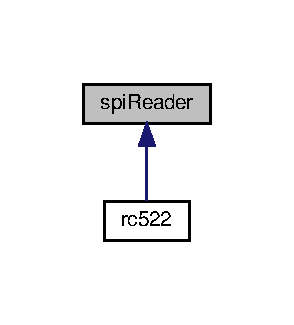
\includegraphics[width=141pt]{classspiReader__inherit__graph}
\end{center}
\end{figure}
\subsection*{Public Types}
\begin{DoxyCompactItemize}
\item 
enum \hyperlink{classspiReader_a4bcf984823c38cf4841ebf619e788790}{status} \{ \newline
{\bfseries E\+R\+R\+OR} = 0x00, 
{\bfseries F\+A\+I\+L\+E\+D\+\_\+\+A\+U\+TH}, 
{\bfseries S\+U\+C\+C\+E\+SS}, 
{\bfseries S\+U\+C\+C\+E\+S\+S\+\_\+\+N\+E\+WC}, 
\newline
{\bfseries S\+U\+C\+C\+E\+S\+S\+\_\+\+O\+L\+DC}, 
{\bfseries T\+I\+M\+E\+O\+U\+T\+C\+OM}, 
{\bfseries T\+I\+M\+E\+O\+U\+T\+D\+EV}, 
{\bfseries T\+I\+M\+E\+O\+UT}, 
\newline
{\bfseries N\+O\+\_\+\+S\+P\+A\+CE}, 
{\bfseries C\+R\+C\+\_\+\+E\+R\+R\+OR}, 
{\bfseries C\+R\+C\+\_\+\+S\+U\+C\+C\+E\+SS}, 
{\bfseries R\+E\+A\+DY}
 \}\begin{DoxyCompactList}\small\item\em A status enum class. \end{DoxyCompactList}
\end{DoxyCompactItemize}
\subsection*{Public Member Functions}
\begin{DoxyCompactItemize}
\item 
\hyperlink{classspiReader_af8eca236eb5cfe4e806f0151227e42b4}{spi\+Reader} (hwlib\+::target\+::pin\+\_\+out \&nss\+Input, hwlib\+::spi\+\_\+bus\+\_\+bit\+\_\+banged\+\_\+sclk\+\_\+mosi\+\_\+miso \&spi\+Bus\+Input)
\begin{DoxyCompactList}\small\item\em The default constructor. \end{DoxyCompactList}\end{DoxyCompactItemize}
\subsection*{Protected Attributes}
\begin{DoxyCompactItemize}
\item 
hwlib\+::target\+::pin\+\_\+out \& \hyperlink{classspiReader_a2a241a80ce921c4df38b3080d839850f}{nss}
\begin{DoxyCompactList}\small\item\em A nss hwlib pin\+\_\+out by ref. \end{DoxyCompactList}\item 
hwlib\+::spi\+\_\+bus\+\_\+bit\+\_\+banged\+\_\+sclk\+\_\+mosi\+\_\+miso \hyperlink{classspiReader_adb87e7c8ca2a11337b67fe8efce50262}{spi\+Bus}
\begin{DoxyCompactList}\small\item\em A spi\+Bus hwlib spi\+\_\+bus\+\_\+bit\+\_\+banged\+\_\+sclk\+\_\+mosi\+\_\+miso. \end{DoxyCompactList}\end{DoxyCompactItemize}


\subsection{Detailed Description}
\hyperlink{classspiReader}{spi\+Reader} A\+DT class 

A A\+DT class for a reader that implements S\+PI, built using hwlib./n You need to supply a hwlib pin\+\_\+out for the nss pin,/n you also has to supply a hwlib spi\+\_\+bus\+\_\+banged\+\_\+sclk\+\_\+mosi\+\_\+miso bus for the spi\+Bus./n You also has to define the read and write funcions when you inherit from this class. 

\subsection{Member Enumeration Documentation}
\mbox{\Hypertarget{classspiReader_a4bcf984823c38cf4841ebf619e788790}\label{classspiReader_a4bcf984823c38cf4841ebf619e788790}} 
\index{spi\+Reader@{spi\+Reader}!status@{status}}
\index{status@{status}!spi\+Reader@{spi\+Reader}}
\subsubsection{\texorpdfstring{status}{status}}
{\footnotesize\ttfamily enum \hyperlink{classspiReader_a4bcf984823c38cf4841ebf619e788790}{spi\+Reader\+::status}\hspace{0.3cm}{\ttfamily [strong]}}



A status enum class. 

This enum class contains all the various statusses the function return. 

\subsection{Constructor \& Destructor Documentation}
\mbox{\Hypertarget{classspiReader_af8eca236eb5cfe4e806f0151227e42b4}\label{classspiReader_af8eca236eb5cfe4e806f0151227e42b4}} 
\index{spi\+Reader@{spi\+Reader}!spi\+Reader@{spi\+Reader}}
\index{spi\+Reader@{spi\+Reader}!spi\+Reader@{spi\+Reader}}
\subsubsection{\texorpdfstring{spi\+Reader()}{spiReader()}}
{\footnotesize\ttfamily spi\+Reader\+::spi\+Reader (\begin{DoxyParamCaption}\item[{hwlib\+::target\+::pin\+\_\+out \&}]{nss\+Input,  }\item[{hwlib\+::spi\+\_\+bus\+\_\+bit\+\_\+banged\+\_\+sclk\+\_\+mosi\+\_\+miso \&}]{spi\+Bus\+Input }\end{DoxyParamCaption})}



The default constructor. 

You need to supply the nss pin\+\_\+out pin and the spi\+Bus spi\+\_\+bus\+\_\+bit\+\_\+banged\+\_\+sclk\+\_\+mosi\+\_\+miso/n since there are no default values. 

\subsection{Member Data Documentation}
\mbox{\Hypertarget{classspiReader_a2a241a80ce921c4df38b3080d839850f}\label{classspiReader_a2a241a80ce921c4df38b3080d839850f}} 
\index{spi\+Reader@{spi\+Reader}!nss@{nss}}
\index{nss@{nss}!spi\+Reader@{spi\+Reader}}
\subsubsection{\texorpdfstring{nss}{nss}}
{\footnotesize\ttfamily hwlib\+::target\+::pin\+\_\+out\& spi\+Reader\+::nss\hspace{0.3cm}{\ttfamily [protected]}}



A nss hwlib pin\+\_\+out by ref. 

A nss hwlib pin\+\_\+out pin used with reference./n The signal nss is used for to be able to send datastreams./n \mbox{\Hypertarget{classspiReader_adb87e7c8ca2a11337b67fe8efce50262}\label{classspiReader_adb87e7c8ca2a11337b67fe8efce50262}} 
\index{spi\+Reader@{spi\+Reader}!spi\+Bus@{spi\+Bus}}
\index{spi\+Bus@{spi\+Bus}!spi\+Reader@{spi\+Reader}}
\subsubsection{\texorpdfstring{spi\+Bus}{spiBus}}
{\footnotesize\ttfamily hwlib\+::spi\+\_\+bus\+\_\+bit\+\_\+banged\+\_\+sclk\+\_\+mosi\+\_\+miso spi\+Reader\+::spi\+Bus\hspace{0.3cm}{\ttfamily [protected]}}



A spi\+Bus hwlib spi\+\_\+bus\+\_\+bit\+\_\+banged\+\_\+sclk\+\_\+mosi\+\_\+miso. 

A spi\+Bus hwlib spi\+\_\+bus\+\_\+bit\+\_\+banged\+\_\+sclk\+\_\+mosi\+\_\+miso,/n the user has to create a spi\+\_\+bus\+\_\+bit\+\_\+banged\+\_\+sclk\+\_\+mosi\+\_\+miso containing a sclk, mosi and miso,/n and supply it to this class. 

The documentation for this class was generated from the following files\+:\begin{DoxyCompactItemize}
\item 
reader.\+hpp\item 
reader.\+cpp\end{DoxyCompactItemize}

%--- End generated contents ---

% Index
\backmatter
\newpage
\phantomsection
\clearemptydoublepage
\addcontentsline{toc}{chapter}{Index}
\printindex

\end{document}
